%%%%%%%%%%%%%%%%%%%%%%%%%%%%%%%%%%%%%%%%%%%%%%%%%%%%%%%%%%%%%%%%%%%%%%%%%%%%%%%%
% PREAMBLE
%%%%%%%%%%%%%%%%%%%%%%%%%%%%%%%%%%%%%%%%%%%%%%%%%%%%%%%%%%%%%%%%%%%%%%%%%%%%%%%%
\documentclass[12pt, a4paper]{article}

% --- PACKAGE IMPORTS ---

% Font and Encoding
\usepackage[utf8]{inputenc}
\usepackage{amsmath}
\usepackage{amssymb} % Provides \mathbb and additional math symbols
\usepackage{times} % Use Times New Roman font family
\usepackage{graphicx} % Required for \includegraphics
\usepackage{booktabs} % Provides \toprule, \midrule, \bottomrule for tables

% Page Layout and Spacing
\usepackage[margin=1in]{geometry}
\linespread{1.1} % Slightly increase line spacing for readability

% Author and Affiliation Formatting
\usepackage{authblk}
\renewcommand\Authfont{\normalsize}
\renewcommand\Affilfont{\small\itshape}
\renewcommand\Authands{, }

% Hyperlinks (for clickable email addresses)
\usepackage{hyperref}
\hypersetup{
    colorlinks=true,
    linkcolor=black,
    urlcolor=blue,
    citecolor=black
}

% List Customization (for the Table of Contents)
\usepackage{enumitem}
% Customize first level enumeration: Bold number with a period
\setlist[enumerate,1]{label=\textbf{\arabic*.}, leftmargin=*}
% Customize second level enumeration: e.g., 1.1, 1.2
\setlist[enumerate,2]{label=\theenumi.\arabic*., leftmargin=*}

% --- BIBLIOGRAPHY (APA STYLE) ---
% Using biblatex for modern and flexible citation management
\usepackage[style=apa, backend=biber]{biblatex}
\addbibresource{references.bib} % Create a file named "references.bib" for your citations

%%%%%%%%%%%%%%%%%%%%%%%%%%%%%%%%%%%%%%%%%%%%%%%%%%%%%%%%%%%%%%%%%%%%%%%%%%%%%%%%
% DOCUMENT METADATA
%%%%%%%%%%%%%%%%%%%%%%%%%%%%%%%%%%%%%%%%%%%%%%%%%%%%%%%%%%%%%%%%%%%%%%%%%%%%%%%%
\title{\bfseries\Large Book Chapter Proposal \\ \vspace{0.3cm}
       \large Beyond Self-Attention: Designing Lightweight Transformer-Like Models with 1D-Convolutions for Green AI}

\author[1]{Ayush Shukla}
\author[1]{Vijay Dwivedi}
\author[2]{Sulabh Sachan}
\author[3]{Iwona Grobelna}
\author[1]{Praveen Pratap Singh}

\affil[1]{Department of Computer Science \& Engineering, United College of Engineering \& Research, Prayagraj, Uttar Pradesh, 211010, India}
\affil[2]{Department of Electrical, IT and Cybernetics, University of South-Eastern Norway, Porsgrunn, Norway}
\affil[3]{Institute of Automatic Control, Electronics and Electrical Engineering, University of Zielona Góra, 65-516 Zielona Góra, Poland}

\date{December 03, 2025}

%%%%%%%%%%%%%%%%%%%%%%%%%%%%%%%%%%%%%%%%%%%%%%%%%%%%%%%%%%%%%%%%%%%%%%%%%%%%%%%%
% BEGIN DOCUMENT
%%%%%%%%%%%%%%%%%%%%%%%%%%%%%%%%%%%%%%%%%%%%%%%%%%%%%%%%%%%%%%%%%%%%%%%%%%%%%%%%
\begin{document}

\maketitle
\thispagestyle{empty} % Removes page number from the title page

% Add a block for contact emails at the bottom of the first page for clarity
\begin{NoHyper} % Prevents hyperref warnings for duplicate targets
\renewcommand{\thefootnote}{\fnsymbol{footnote}}
\footnotetext[1]{Corresponding Emails: 
\href{mailto:shuklaayush0704@gmail.com}{\texttt{shuklaayush0704@gmail.com}}, 
\href{mailto:vijaydwivedi@united.ac.in}{\texttt{vijaydwivedi@united.ac.in}}, 
\href{mailto:sulabh.sachan@usn.no}{\texttt{sulabh.sachan@usn.no}}, 
\href{mailto:i.grobelna@iee.uz.zgora.pl}{\texttt{i.grobelna@iee.uz.zgora.pl}}, 
\href{mailto:praveenpratapsingh@united.ac.in}{\texttt{praveenpratapsingh@united.ac.in}}
}
\renewcommand{\thefootnote}{\arabic{footnote}}
\end{NoHyper}

% --- ABSTRACT ---
\section*{Abstract}
\noindent % No indent for the first line
The increasing computational demands of state-of-the-art deep learning models, particularly Transformers, present a significant challenge to the goal of sustainable, or "Green,” AI. While hybrid architectures have advanced computer vision, their core self-attention mechanisms remain a major source of parameter and computational inefficiency. This chapter directly addresses this challenge by exploring architectural innovations that move beyond self-attention. We introduce \textbf{EcoConvNet}, a novel and lightweight Transformer-like architecture meticulously designed for energy-efficient computer vision. The central innovation of our model is the replacement of the canonical Multi-Head Self-Attention block with a highly efficient sequence processor built on temporal 1D-Convolutions. This design choice drastically reduces the model's complexity from quadratic to linear with respect to sequence length, leading to substantial gains in efficiency. We further enhance the architecture with a unique Positional-Biased Attention Pooling mechanism, a parameter-efficient module that integrates content-based feature importance with a learnable spatial bias. Through rigorous empirical evaluation, we demonstrate that EcoConvNet achieves a superior accuracy-per-FLOP trade-off compared to conventional baselines. This work provides a concrete design paradigm for developing next-generation Green AI models that are both powerful and computationally sustainable, making them suitable for deployment in resource-constrained environments.

\vspace{0.3cm}

% --- KEYWORDS ---
\noindent\textbf{Keywords:} Energy-Efficient Architectures, Sustainable Deep Learning, Green AI, Hybrid Vision Models, Lightweight Transformers, 1D-Convolutions.

\vspace{0.5cm}
\hrulefill % Adds a horizontal line to visually separate the abstract from the main content
\vspace{0.5cm}

% --- DETAILED TABLE OF CONTENTS ---
\section*{Detailed Table of Contents}

\begin{enumerate}
    \item \large\bfseries Introduction to Sustainable Deep Learning \\
    \normalfont This introductory section will set the stage by discussing the growing carbon footprint of the AI industry. We will define the concept of "Green AI" and argue for the critical importance of developing energy-efficient models.
    \begin{enumerate}
        \item \textit{The Computational Cost of Modern AI:} We will present key statistics and studies on the energy consumption associated with training large-scale models.
        \item \textit{The Rise of Green AI: Principles and Objectives:} This subsection will formalize the goals of Green AI, focusing on metrics beyond accuracy, such as FLOPs, parameter count, and inference latency.
        \item \textit{The Role of Energy-Efficient Architectures:} We will introduce the central thesis of the chapter: that architectural innovation is a primary driver of sustainability in deep learning.
        \item \textit{Chapter Motivation and Outline:} The section will conclude with the specific motivation for our work—the need for efficient alternatives to self-attention—and provide a roadmap for the rest of the chapter.
    \end{enumerate}

    \item \large\bfseries Background: The Evolution of Efficient Vision Architectures \\
    \normalfont This section will provide a pedagogical review of key architectural developments, creating a foundation for understanding our proposed model.
    \begin{enumerate}
        \item \textit{The Era of CNNs: From AlexNet to EfficientNet:} A historical overview of landmark CNN architectures, with a focus on design principles that improved efficiency.
        \item \textit{The Transformer Revolution in Computer Vision:} This subsection will deconstruct the seminal Vision Transformer (ViT) architecture and critically analyze its quadratic complexity as its primary efficiency bottleneck.
        \item \textit{State-of-the-Art in Hybrid and Efficient Models:} A review of models that merge CNN and Transformer concepts, highlighting their strengths and remaining efficiency challenges.
    \end{enumerate}
    
    \item \large\bfseries Methodology: Designing the EcoConvNet Architecture \\
    \normalfont This is the core technical section of the chapter, where we will present our novel architecture in detail. Architectural diagrams and pseudo-code will be used for clarity.
    \begin{enumerate}
        \item \textit{Overall Architectural Blueprint:} A high-level diagram and description of the complete model pipeline.
        \item \textit{The CNN Backbone for Efficient Feature Extraction:} We will detail the lightweight CNN front-end used to generate spatially rich feature maps.
        \item \textit{A Lightweight Alternative to Self-Attention: The 1D-Convolutional Sequence Processor:} This subsection presents our first key contribution, contrasting its linear complexity with the quadratic complexity of MHSA.
        \item \textit{Novelty Focus: The Positional-Biased Attention Pooling Mechanism:} This subsection details our second key contribution, explaining its mathematical formulation and intuition.
    \end{enumerate}

    \item \large\bfseries Experimental Evaluation and Analysis \\
    \normalfont This section will be dedicated to the empirical validation of our proposed architecture, providing quantitative evidence of its efficiency and effectiveness.
    \begin{enumerate}
        \item \textit{Datasets and Evaluation Metrics:} We will describe the datasets used (e.g., MNIST, CIFAR-10/100) and formally define the sustainability metrics.
        \item \textit{Baselines for Comparison:} We will outline the baseline models (e.g., standard CNNs, ResNet) for a fair and comprehensive evaluation.
        \item \textit{Performance Analysis: The Accuracy vs. Efficiency Trade-off:} The main results will be presented using tables and Pareto-optimality plots (Accuracy vs. GFLOPs).
        \item \textit{Ablation Studies: Validating Architectural Choices:} Crucial experiments to isolate the impact of our novel components.
    \end{enumerate}

    \item \large\bfseries Discussion, Future Work, and Broader Impact \\
    \normalfont In this concluding section, we will interpret our findings, discuss their implications, and suggest avenues for future research.
    \begin{enumerate}
        \item \textit{Interpreting the Results: Why EcoConvNet is Efficient:} A qualitative discussion on how our design choices lead to the observed performance gains.
        \item \textit{Implications for Edge AI and the Internet of Things (IoT):} We will discuss the real-world applicability of our model for on-device machine learning.
        \item \textit{Future Research Directions:} We will propose future work, including model quantization, neural architecture search, and adapting the architecture for other tasks.
    \end{enumerate}

    \item \large\bfseries Conclusion \\
    \normalfont A summary of the chapter's key findings, restating the contribution of our work to the field of sustainable deep learning and energy-efficient architectures.

    \item \large\bfseries References \\
    \normalfont A comprehensive list of 55-90 references in APA style will be provided in the full chapter submission, citing all relevant foundational and state-of-the-art works.
\end{enumerate}





%%%%%%%%%%%%%%%%%%%%%%%%%%%%%%%%%%%%%%%%%%%%%%%%%%%%%%%%%%%%%%%%%%%%%%%%%%%%%%%%
% CHAPTER 1: INTRODUCTION
%%%%%%%%%%%%%%%%%%%%%%%%%%%%%%%%%%%%%%%%%%%%%%%%%%%%%%%%%%%%%%%%%%%%%%%%%%%%%%%%

\section{Introduction to Sustainable Deep Learning}
\label{sec:introduction}

The last decade has witnessed a paradigm shift in artificial intelligence, largely driven by the unprecedented success of deep learning. Architectures such as the Transformer \cite{vaswani2017attention} have achieved state-of-the-art performance across a breathtaking array of domains, from natural language processing and computer vision to scientific discovery and drug design \cite{jumper2021highly}. This revolution, fueled by massive datasets and vast computational resources, has ushered in an era of models with hundreds of billions of parameters, such as GPT-3 \cite{brown2020language} and PaLM \cite{chowdhery2022palm}, capable of tasks once considered the exclusive domain of human intelligence.

However, this monumental progress has come at a steep, often unacknowledged, computational and environmental price. The dominant research paradigm, frequently termed "Red AI" \cite{schwartz2020green}, has prioritized predictive accuracy above all else, leading to a computational arms race where bigger models are axiomatically assumed to be better. This trend is fundamentally unsustainable, especially in an era where the performance gains from Moore's Law have decelerated, meaning we can no longer rely on hardware improvements alone to manage escalating computational demands \cite{hennessy2019new}. This introductory chapter sets the stage for our work by first quantifying the staggering cost of modern AI and then introducing the principles of Green AI, a responsive movement advocating for efficiency as a primary scientific objective. We argue that the most impactful path toward a sustainable AI future lies not just in optimizing existing models, but in fundamental architectural innovation that moves beyond the computationally expensive primitives of today's leading architectures.

\subsection{The Computational Cost of Modern AI}
\label{ssec:computational_cost}

The escalation in the scale of deep learning models has led to an exponential increase in their computational demands and, consequently, their carbon footprint. The process of training a single large-scale Transformer model can be astonishingly energy-intensive. A landmark study by Strubell et al. \cite{strubell2019energy} revealed that training a single large NLP model via neural architecture search could emit as much carbon as five cars over their entire lifetimes, including fuel---an amount equivalent to over 300 round-trip flights between New York and San Francisco. More critically, their analysis demonstrated that training a Transformer-based model with neural architecture search consumed approximately 284 tons of CO$_2$ equivalent, highlighting the environmental toll of modern AI development \cite{bender2021dangers}.

While this study highlighted a worst-case scenario, more recent analyses from industry leaders confirm the severity of the issue. Patterson et al. \cite{patterson2021carbon} from Google provided a detailed account of the carbon emissions associated with training major models like T5 \cite{raffel2020exploring}, noting that while factors like data center energy efficiency and geographical location play a significant role, the total energy consumption remains a major concern. The training of their 11-billion-parameter T5 model, for instance, consumed energy on the order of hundreds of MWh (megawatt-hours). These figures represent only the \textit{final training run}; they exclude the countless experiments, hyperparameter tuning, and preliminary model developments that constitute the bulk of the research and development lifecycle. Recent estimates suggest that training GPT-3, with its 175 billion parameters, consumed approximately 1,287 MWh and generated over 550 tons of CO$_2$ emissions \cite{luccioni2022estimating}.

The computational intensity problem extends beyond training to inference at scale. Large language models deployed in production systems, such as ChatGPT serving millions of daily queries, incur substantial ongoing energy costs \cite{wu2022sustainable}. A single inference pass through GPT-3 scale models can require several kilowatt-hours, and when aggregated across billions of queries, the cumulative environmental impact becomes staggering \cite{dodge2022measuring}. This operational carbon footprint often exceeds training emissions over the model's lifetime, yet receives comparatively less attention in the literature \cite{gupta2022chasing}.

This trend toward computationally extravagant models creates not only an environmental challenge but also an equity and accessibility crisis. When the cost of training a state-of-the-art model from scratch runs into millions of dollars, research becomes increasingly concentrated in the hands of a few large, well-funded technology corporations \cite{ahmed2022utility}. This dynamic stifles innovation in academia and smaller organizations, hindering the democratization of AI \cite{birhane2022values}. The pursuit of ever-larger models is, therefore, on a collision course with both ecological limits and the principles of open scientific inquiry. Furthermore, the energy requirements pose significant barriers to deploying AI solutions in resource-constrained environments and developing regions where computational infrastructure is limited \cite{hershcovich2022towards}.

\subsection{The Rise of Green AI: Principles and Objectives}
\label{ssec:green_ai_principles}

In response to this escalating crisis, the research community has begun to champion a new paradigm: \textbf{Green AI} \cite{schwartz2020green}. Green AI reframes the goals of AI research, proposing that efficiency should be a first-order evaluation metric alongside accuracy. It encourages a shift in focus from achieving marginal gains on benchmark leaderboards at any cost to developing models that are computationally frugal, accessible, and sustainable. The principles of Green AI are formalized through a new set of objectives and evaluation metrics that extend beyond simple task performance \cite{menghani2023efficient}. This paradigm shift aligns with broader sustainability initiatives in computing, where the carbon intensity of machine learning workflows is increasingly scrutinized \cite{verdecchia2023systematic}.

The key objectives of Green AI are to minimize the resources required for both training and inference, which can be measured through several complementary metrics:

\begin{itemize}
    \item \textbf{Computational Complexity (FLOPs):} Floating Point Operations (FLOPs) measure the total number of arithmetic operations a model performs to process a single input. It is a hardware-agnostic metric that provides a standardized estimate of a model's computational cost. A primary goal of Green AI is to design architectures that achieve high accuracy with a minimal number of FLOPs, often reported in GFLOPs (billions of FLOPs). The quadratic complexity of self-attention in Transformers \cite{dosovitskiy2020image} is a primary target for reduction. Recent work has established that reducing FLOPs by even 10\% can translate to measurable energy savings across large-scale deployments \cite{desislavov2023compute}.

    \item \textbf{Parameter Count and Model Size:} The number of trainable parameters in a model directly correlates with its memory requirements for storage and deployment. Models with fewer parameters, such as MobileNets \cite{howard2017mobilenets} and EfficientNets \cite{tan2019efficientnet}, are not only faster to train but are also essential for deployment on resource-constrained edge devices like mobile phones and IoT sensors, where memory and power are limited. Efficient parameter utilization also facilitates model distribution and reduces bandwidth requirements for over-the-air updates in distributed systems \cite{cai2020once}.

    \item \textbf{Inference Latency:} This metric measures the real-world time it takes for a trained model to make a prediction on a given hardware platform (e.g., CPU, GPU, or TPU). Low latency is critical for real-time applications such as autonomous navigation, real-time language translation, and interactive user interfaces. Hardware-aware neural architecture search has emerged as a promising approach to optimize latency while maintaining accuracy \cite{cai2019proxylessnas, wu2019fbnet}.

    \item \textbf{Energy Consumption:} The most direct measure of a model's environmental impact is its total energy usage, typically measured in joules or kilowatt-hours (kWh). While this is the most important metric, it is hardware-dependent and often difficult to measure directly \cite{garcia2019estimation}, which is why proxies like FLOPs and model size are commonly used in research. Recent tools and frameworks, such as CodeCarbon and ML CO2 Impact, have enabled more systematic energy profiling of machine learning workloads \cite{lacoste2019quantifying, anthony2020carbontracker}.

    \item \textbf{Accuracy-Efficiency Trade-offs:} Modern Green AI research emphasizes Pareto-optimal architectures that maximize predictive performance per unit of computational resource. The concept of "efficiency frontiers" has become central to model evaluation, where models are compared not by accuracy alone but by their position on the accuracy-vs-FLOPs curve \cite{dehghani2021efficiency}. This holistic evaluation framework ensures that efficiency gains are not achieved at the expense of unacceptable performance degradation.
\end{itemize}



\subsection{The Role of Energy-Efficient Architectures}
\label{ssec:role_of_architectures}

Addressing the sustainability challenge in AI requires a multi-faceted approach, including improvements in hardware, data center efficiency, and algorithmic optimization. However, we posit that the most fundamental and impactful driver of sustainability is \textbf{architectural innovation}. While techniques such as network pruning \cite{han2015deep}, quantization \cite{gholami2022survey}, and knowledge distillation \cite{hinton2015distilling} are valuable for compressing trained models, they often act as post-hoc optimizations on an already inefficient foundation. These methods trim the branches of a computationally expensive tree, whereas architectural innovation redesigns the tree from its roots to be inherently more efficient. Structured pruning methods \cite{liu2017learning} and dynamic neural networks \cite{han2021dynamic} represent advances in this direction, but fundamental architectural redesign often yields the most substantial gains.

The history of deep learning provides compelling evidence for this thesis. The initial breakthrough in computer vision with AlexNet \cite{krizhevsky2012imagenet} was followed by architectures like VGGNet \cite{simonyan2014very}, which achieved higher accuracy at the cost of immense parameter counts. A significant architectural shift occurred with the introduction of Residual Networks (ResNets) \cite{he2016deep}, which enabled deeper, more powerful models without succumbing to vanishing gradients. An even greater leap in efficiency came from fundamentally rethinking the core convolutional operator. The depthwise separable convolutions introduced in MobileNets \cite{howard2017mobilenets} drastically reduced the FLOPs and parameter count of standard convolutions, setting a new precedent for lightweight design. More recently, EfficientNet \cite{tan2019efficientnet} demonstrated that a principled approach to scaling model depth, width, and resolution could yield a superior trade-off between accuracy and efficiency.

In each of these cases, the most substantial gains in the accuracy-per-FLOP trade-off were not achieved by compressing a large model, but by designing a new, more computationally frugal building block. This principle is more critical than ever in the era of Transformers. While the self-attention mechanism is remarkably effective at modeling long-range dependencies, its quadratic complexity with respect to input sequence length makes it a prime candidate for architectural disruption. Efficient attention mechanisms, including linear attention \cite{katharopoulos2020transformers}, sparse attention patterns \cite{child2019generating}, and low-rank approximations \cite{wang2020linformer}, have demonstrated the viability of reducing computational complexity while preserving much of the representational power of full attention. Furthermore, hybrid architectures that strategically combine convolutions with attention \cite{dai2021coatnet, wang2021pyramid} have shown that architectural diversity can yield significant efficiency benefits.

The emergence of Neural Architecture Search (NAS) \cite{zoph2018learning, elsken2019neural} has provided a systematic framework for discovering efficient architectures, yet the search space design itself remains an open problem. Hardware-aware NAS \cite{cai2019proxylessnas, tan2021efficientnetv2} extends this paradigm by optimizing directly for target deployment platforms, acknowledging that FLOPs alone do not fully capture real-world efficiency. Therefore, the path toward a truly Green AI lies in developing novel architectural primitives that can replicate the successes of the Transformer without inheriting its computational extravagance, while also considering the co-design of algorithms and hardware \cite{chen2019tvm}.

\subsection{Chapter Motivation and Outline}
\label{ssec:motivation_and_outline}

The central motivation for this chapter is to address the primary efficiency bottleneck of the Vision Transformer (ViT) \cite{dosovitskiy2020image} and its many variants: the self-attention mechanism. When an image is partitioned into a sequence of patches, a standard-sized input of $224 \times 224$ pixels with $16 \times 16$ patches results in a sequence of length $N=196$. The computational cost of self-attention, which scales as $O(N^2)$, becomes prohibitive for higher-resolution images and computationally constrained devices. For instance, processing a $1024 \times 1024$ image would result in a sequence length of $N=4096$, leading to a 16-fold increase in computational cost compared to standard resolution—a scaling that is untenable for real-time applications and edge deployment \cite{liu2021swin}.

While numerous works have proposed approximations to make attention more efficient, such as Linformer \cite{wang2020linformer}, Performer \cite{choromanski2020rethinking}, and Nyströmformer \cite{xiong2021nystromformer}, many still struggle to match the performance of the original formulation or introduce other complexities. Sparse attention mechanisms \cite{child2019generating, zaheer2020big} reduce computational cost by attending to only a subset of tokens, but require careful design to avoid information loss. Hierarchical architectures like Swin Transformer \cite{liu2021swin} achieve linear complexity through windowed attention but sacrifice true global receptive fields in early layers.

More recently, a new wave of research has begun to question whether self-attention is necessary for state-of-the-art performance. Architectures like MLP-Mixer \cite{tolstikhin2021mlp}, FNet \cite{leethorp2021fnet}, and ConvNeXt \cite{liu2022convnet} have demonstrated that carefully designed MLP-based, Fourier-based, or pure-convolutional models can outperform Transformers, suggesting that the general meta-architecture of Transformers (e.g., patch-based processing, stacked blocks, normalization strategies) may be as important as the attention mechanism itself \cite{yu2022metaformer}. The success of these attention-free models raises a compelling research question: Can we design a novel, linear-time sequence processor that preserves the powerful feature-learning capabilities of Transformer-like models while being explicitly optimized for computational efficiency?

This chapter directly addresses this question by introducing \textbf{EcoConvNet}, a lightweight, hybrid vision architecture. Our core contribution is the replacement of the quadratic-cost Multi-Head Self-Attention (MHSA) block with a highly efficient 1D-Convolutional Sequence Processor, which reduces the complexity from $O(N^2)$ to linear $O(N)$ with respect to sequence length. This design choice is motivated by recent findings that temporal convolutions can effectively model sequential dependencies in vision tasks \cite{bai2018empirical, vaswani2021scaling}, while offering superior computational efficiency and hardware compatibility. Our approach is complemented by a novel Positional-Biased Attention Pooling mechanism designed to capture global spatial information with minimal overhead, drawing inspiration from recent advances in efficient pooling strategies \cite{jaegle2021perceiver}.

Our work provides a concrete design paradigm for building next-generation Green AI models that are suitable for deployment in resource-constrained environments, such as those found in Edge AI and the Internet of Things (IoT) \cite{verhelst2020machine, li2021survey}. The architectural innovations presented in this chapter are guided by three core principles: (1) \textit{complexity reduction} through linear-time operations, (2) \textit{parameter efficiency} via strategic weight sharing and factorization, and (3) \textit{hardware awareness} by favoring operations with optimized implementations on common accelerators \cite{sze2017efficient}. By adhering to these principles, EcoConvNet achieves a favorable balance between accuracy, efficiency, and deployability that positions it as a viable alternative to conventional Transformer-based vision models for sustainability-conscious applications.


%To guide the reader, the remainder of this chapter is structured as follows:
%\begin{itemize}
 %   \item \textbf{Chapter 2} provides a pedagogical review of the evolution of vision architectures, from the foundational principles of CNNs to the rise of Vision Transformers and the latest generation of efficient hybrid models, establishing the context for our work.
%    \item \textbf{Chapter 3} presents the core technical contribution, detailing the architectural blueprint of EcoConvNet. We provide mathematical formulations, diagrams, and pseudo-code for our novel components.
 %   \item \textbf{Chapter 4} is dedicated to our empirical evaluation. We present a rigorous comparison of EcoConvNet against state-of-the-art baselines on standard computer vision benchmarks, focusing on the trade-off between accuracy and efficiency metrics.
  %  \item \textbf{Chapter 5} discusses the broader implications of our results, interpreting why EcoConvNet is efficient and exploring its applications and avenues for future research.
   % \item \textbf{Chapter 6} concludes the chapter with a summary of our key findings and contributions to the field of sustainable deep learning.
%\end{itemize}




%%%%%%%%%%%%%%%%%%%%%%%%%%%%%%%%%%%%%%%%%%%%%%%%%%%%%%%%%%%%%%%%%%%%%%%%%%%%%%%%
% CHAPTER 2: BACKGROUND
%%%%%%%%%%%%%%%%%%%%%%%%%%%%%%%%%%%%%%%%%%%%%%%%%%%%%%%%%%%%%%%%%%%%%%%%%%%%%%%%

\section{Background: The Evolution of Efficient Vision Architectures}
\label{sec:background}

To fully appreciate the motivation and design of EcoConvNet, it is essential to trace the architectural evolution of deep learning models for computer vision. This history is not merely a sequence of incremental improvements but a story of paradigm shifts, where fundamental design principles were challenged and reinvented in the pursuit of greater performance and efficiency. This section provides a pedagogical review of the two major eras that define the modern landscape: the rise and refinement of Convolutional Neural Networks (CNNs), and the subsequent revolution brought about by Transformers.

\subsection{The Era of CNNs: From AlexNet to EfficientNet}
\label{ssec:cnn_era}

The modern era of deep learning for computer vision was ignited in 2012 when AlexNet \cite{krizhevsky2012imagenet} demonstrated a monumental leap in performance on the ImageNet Large Scale Visual Recognition Challenge. Its architecture, while computationally demanding for its time, established a foundational blueprint: a sequence of convolutional layers to extract hierarchical features, interspersed with pooling layers for spatial downsampling, and followed by fully-connected layers for classification. This success was amplified by the use of the Rectified Linear Unit (ReLU) activation function \cite{nair2010rectified} and GPU acceleration, which became standard practice. AlexNet's introduction of dropout regularization \cite{srivastava2014dropout} and data augmentation techniques also set new standards for preventing overfitting in deep networks.

Following this breakthrough, the immediate trend was a push toward deeper networks in a brute-force quest for higher accuracy. VGGNet \cite{simonyan2014very} epitomized this philosophy by stacking many layers of small, 3x3 convolutional filters, demonstrating that network depth was a critical factor in learning rich representations. While VGG's uniform structure was elegant and powerful, its immense parameter count (138 million parameters in VGG-16) and computational cost highlighted the limitations of simply scaling depth naively. This "deeper is better" approach soon hit a wall due to the vanishing gradient problem, which made training extremely deep networks prohibitively difficult \cite{glorot2010understanding}.

The first major architectural innovation to overcome this barrier was the Residual Network (ResNet) \cite{he2016deep}. ResNet introduced the concept of a "residual connection" or "skip connection," a simple identity mapping that allowed gradients to bypass layers and flow more easily during backpropagation. This elegant solution enabled the training of networks with hundreds or even thousands of layers, leading to new states of the art. The mathematical formulation $\mathbf{y} = \mathcal{F}(\mathbf{x}) + \mathbf{x}$ transformed the learning objective from modeling $\mathcal{H}(\mathbf{x})$ directly to learning a residual function $\mathcal{F}(\mathbf{x}) = \mathcal{H}(\mathbf{x}) - \mathbf{x}$, which empirically proved easier to optimize. The success of ResNet, alongside techniques like Batch Normalization \cite{ioffe2015batch}, demonstrated that clever architectural design, rather than raw depth alone, was key to unlocking performance.

Concurrently, the GoogLeNet architecture introduced the Inception module \cite{szegedy2015going}, which used parallel convolutional filters of different sizes (1x1, 3x3, 5x5) and 1x1 convolutions as bottleneck layers to reduce computational cost while capturing multi-scale features. This design philosophy of using multi-branch architectures was further refined in Inception-v2 \cite{ioffe2015batch}, Inception-v3 \cite{szegedy2016rethinking}, and Inception-v4 \cite{szegedy2017inception}, each introducing incremental improvements in efficiency and accuracy. The success of Inception architectures demonstrated that architectural diversity within a single model could enhance representational capacity without proportional increases in computational cost.

While ResNet and GoogLeNet made networks more effective, the next paradigm shift was explicitly focused on computational efficiency, particularly for mobile and edge devices. This movement was spearheaded by MobileNet \cite{howard2017mobilenets}, which replaced the standard convolutional layer with the highly efficient \textbf{depthwise separable convolution}. This operation factorizes a standard convolution into two cheaper steps: a depthwise convolution that applies a single filter to each input channel (mixing spatial information), followed by a pointwise (1x1) convolution that combines the outputs (mixing channel information). This decomposition drastically reduces the number of parameters and FLOPs—often by a factor of 8-9x—with only a minor drop in accuracy. Mathematically, for an input of size $D_F \times D_F \times M$ and $N$ output channels with kernel size $D_K$, standard convolution requires $D_K \cdot D_K \cdot M \cdot N \cdot D_F \cdot D_F$ operations, whereas depthwise separable convolution requires only $D_K \cdot D_K \cdot M \cdot D_F \cdot D_F + M \cdot N \cdot D_F \cdot D_F$ operations, yielding a reduction factor of approximately $\frac{1}{N} + \frac{1}{D_K^2}$.

This principle was further refined in architectures like Xception \cite{chollet2017xception}, which pushed depthwise separable convolutions to the extreme, and MobileNetV2 \cite{sandler2018mobilenetv2}, which introduced inverted residual blocks with linear bottlenecks. MobileNetV2's key insight was to expand channels in the middle of the block (inverted residual) and use linear activations in bottleneck layers to preserve information, a design pattern that became influential in subsequent efficient architectures. ShuffleNet \cite{zhang2018shufflenet} further enhanced efficiency by introducing channel shuffle operations to enable cross-group information flow in group convolutions, achieving state-of-the-art accuracy-efficiency trade-offs on mobile devices.

The culmination of this efficiency-focused research was EfficientNet \cite{tan2019efficientnet}. Its authors argued that scaling network dimensions (depth, width, and image resolution) should not be done arbitrarily but in a balanced and principled manner. They introduced "compound scaling," a method that uses a fixed coefficient to uniformly scale all three dimensions according to the relationship: depth $d = \alpha^\phi$, width $w = \beta^\phi$, and resolution $r = \gamma^\phi$, where $\alpha \cdot \beta^2 \cdot \gamma^2 \approx 2$ and $\phi$ is a user-specified coefficient. By starting with a highly efficient baseline architecture discovered through neural architecture search (NAS) \cite{zoph2018learning} and incorporating Squeeze-and-Excitation (SE) blocks \cite{hu2018squeeze} to improve feature quality through channel-wise attention, EfficientNet established a new Pareto-optimal frontier, achieving state-of-the-art accuracy with significantly fewer parameters and FLOPs than previous models. EfficientNet-B7 achieved 84.3\% top-1 accuracy on ImageNet with 66M parameters, compared to GPipe's 84.3\% with 556M parameters, representing an 8.4x parameter reduction. This work represented the zenith of efficient CNN design, demonstrating that a holistic and systematic approach to architecture could yield extraordinary gains. The design principles established in this era—from residual connections and bottleneck layers to depthwise separable convolutions and compound scaling—form the foundation of the CNN backbone used in our proposed EcoConvNet.




\subsection{The Transformer Revolution in Computer Vision}
\label{ssec:transformer_revolution}

While CNNs dominated computer vision for nearly a decade, a revolutionary architecture was emerging from the field of Natural Language Processing (NLP). The Transformer, introduced in the seminal paper "Attention Is All You Need" \cite{vaswani2017attention}, dispensed with recurrence and convolution entirely, relying on a mechanism called \textbf{self-attention} to model global dependencies between input tokens. Its unprecedented success in NLP tasks prompted researchers to adapt it for vision.

The landmark model that successfully translated the Transformer to computer vision was the Vision Transformer (ViT) \cite{dosovitskiy2020image}. The core innovation of ViT was a simple yet effective method for treating an image as a sequence. The image is first split into a grid of non-overlapping patches (e.g., 16x16 pixels). Each patch is flattened into a vector and linearly projected into an embedding space. To retain spatial information, which is lost during patching, learnable positional embeddings are added to these patch embeddings. This sequence of vectors is then fed into a standard Transformer encoder, which consists of a stack of blocks, each containing two main sub-layers: a Multi-Head Self-Attention (MHSA) layer and a position-wise feed-forward network (MLP).

The MHSA layer is the heart of the Transformer's power. For each patch embedding in the sequence, it computes an attention score that determines how much focus to place on all other patches. This allows the model to learn long-range dependencies across the entire image, effectively giving every patch a global receptive field from the very first layer---a stark contrast to the local receptive fields of CNNs. This capability proved immensely powerful, and Transformers quickly set new standards in image classification \cite{touvron2021training} and became the backbone for tasks like object detection \cite{carion2020end} and multi-modal learning \cite{radford2021learning}.

However, this global receptive field comes at a severe computational cost. The self-attention mechanism's complexity is quadratic with respect to the number of input patches, $N$. For an input sequence of length $N$, it must compute an $N \times N$ attention matrix of pairwise scores, resulting in a complexity of $O(N^2 d)$ for embedding dimension $d$. For a standard $224 \times 224$ image with $16 \times 16$ patches, $N=196$. If the image resolution is doubled to $448 \times 448$, the sequence length quadruples to $N=784$, causing the computational cost of the attention layer to increase by a factor of $16$. This quadratic scaling is the primary efficiency bottleneck of the ViT architecture, making it prohibitively expensive for high-resolution imagery and unsuitable for many resource-constrained applications. Empirical studies have shown that self-attention can account for 50-70\% of the total computational budget in Vision Transformers \cite{liu2021swin}.

This fundamental limitation has spurred a wave of research into more efficient model designs. Hierarchical architectures such as Swin Transformer \cite{liu2021swin} and Pyramid Vision Transformer (PVT) \cite{wang2021pyramid} reduce computational complexity by restricting attention to local windows and introducing hierarchical feature pyramids, achieving near-linear complexity while maintaining strong performance. However, these designs sacrifice true global receptive fields in early layers, potentially limiting their ability to capture long-range dependencies. Other approaches, such as Linformer \cite{wang2020linformer}, approximate the full attention matrix using low-rank decomposition, projecting keys and values to a lower dimension to achieve linear complexity. Performer \cite{choromanski2020rethinking} uses random feature approximations to estimate attention scores without explicitly computing the quadratic attention matrix, while Nystr\"{o}mformer \cite{xiong2021nystromformer} employs the Nystr\"{o}m method to approximate the attention matrix using a subset of landmark tokens. Despite these innovations, many efficient attention mechanisms struggle to match the performance of standard self-attention or introduce implementation complexity that limits their practical adoption \cite{tay2022efficient}.

However, this global receptive field comes at a severe computational cost. The self-attention mechanism's complexity is quadratic with respect to the number of input patches, $N$. For an input sequence of length $N$, it must compute an $N \times N$ attention matrix of pairwise scores, resulting in a complexity of $O(N^2)$. For a standard $224 \times 224$ image with $16 \times 16$ patches, $N=196$. If the image resolution is doubled to $448 \times 448$, the sequence length quadruples to $N=784$, causing the computational cost of the attention layer to increase by a factor of $16$. This quadratic scaling is the primary efficiency bottleneck of the ViT architecture, making it prohibitively expensive for high-resolution imagery and unsuitable for many resource-constrained applications. This fundamental limitation has spurred a wave of research into more efficient model designs.

\subsection{State-of-the-Art in Hybrid and Efficient Models}
\label{ssec:hybrid_efficient_models}

In response to the computational demands of pure Transformers, a major research direction has focused on creating hybrid architectures that combine the strengths of both CNNs and Transformers. The rationale is compelling: CNNs are highly efficient at extracting local features and possess a valuable inductive bias (translation equivariance), while Transformers excel at modeling global context. This synergistic approach aims to leverage the complementary strengths of both paradigms while mitigating their respective weaknesses \cite{trockman2023mimetic}.

Early hybrid models often employed a CNN backbone to generate feature maps, which were then fed into a Transformer encoder for final classification, as seen in BoTNet \cite{srinivas2021bottleneck}. More sophisticated designs sought to interleave convolutional and attention-based operations. CoAtNet \cite{dai2021coatnet}, for example, strategically stacked convolutional and self-attention layers, demonstrating that a carefully balanced fusion outperforms either architecture in isolation, achieving 90.88\% top-1 accuracy on ImageNet-1K with only 2.44 GFLOPs. A particularly influential lightweight hybrid is MobileViT \cite{mehta2021mobilevit}, which integrates Transformer blocks into a MobileNet-style backbone. It introduces a novel MobileViT block that uses standard convolutions for local processing before unfolding the feature map into patches for a Transformer to learn global relationships. While highly effective, these models can introduce structural complexity and still rely on the expensive quadratic-time attention mechanism, even if applied to smaller feature maps.

Recent innovations in efficient vision architectures have explored various design spaces. The Twins architecture \cite{chu2021twins} introduces spatially separable self-attention, decomposing the global attention into local and global components for improved efficiency. CrossViT \cite{chen2021crossvit} processes image patches at different scales in parallel and fuses them through cross-attention, enabling more flexible multi-scale feature learning. The concept of token reduction has also gained traction, where methods like Token-to-Token ViT (T2T-ViT) \cite{yuan2021tokens} and DynamicViT \cite{rao2021dynamicvit} progressively reduce the number of tokens in deeper layers, pruning less informative patches to reduce computational cost without significant accuracy loss.

This has led to a more radical line of inquiry that questions the necessity of self-attention itself. This "post-Transformer" movement explores whether the impressive performance of ViTs stems from the attention mechanism or from their general meta-architecture (e.g., the patch-based, block-stacking design) \cite{yu2022metaformer}. The first major challenger was MLP-Mixer \cite{tolstikhin2021mlp}, which replaced the self-attention layer with a simple Multi-Layer Perceptron (MLP). It used one MLP for "token-mixing" (communicating information across different spatial locations) and another for "channel-mixing" (communicating across feature channels), demonstrating surprisingly strong performance. Follow-up works like FNet \cite{leethorp2021fnet} replaced attention with Fourier transforms, while ResMLP \cite{touvron2021resmlp} and gMLP \cite{liu2021pay} further explored MLP-only architectures with spatial gating mechanisms.

Building on this momentum, ConvNeXt \cite{liu2022convnet} provided a powerful counterpoint. The authors modernized a standard ResNet by progressively incorporating design choices from Transformers---such as a patchifying stem (using non-overlapping $4 \times 4$ convolutions), larger kernel sizes (up to $7 \times 7$), inverted bottleneck blocks with depthwise convolutions, GELU activations, and LayerNorm---to create a pure CNN that matched or exceeded the performance of state-of-the-art Transformers like the Swin Transformer \cite{liu2021swin}. The success of ConvNeXt strongly suggests that architectural design principles, rather than a specific mechanism like self-attention, are key to high performance. This has opened the door for other efficient, attention-free alternatives, such as those based on Fourier Transforms like GFNet \cite{rao2021global}, the abstracted MetaFormer concept \cite{yu2022metaformer}, and even simpler pooling-based architectures like PoolFormer \cite{yu2022metaformer}.

The landscape of efficient vision architectures has further diversified with the emergence of techniques that optimize for specific hardware constraints. Hardware-aware neural architecture search (HW-NAS) methods, such as FBNet \cite{wu2019fbnet} and ProxylessNAS \cite{cai2019proxylessnas}, directly optimize for target platforms (e.g., mobile CPUs, GPUs) during the architecture search process, acknowledging that theoretical FLOPs do not always correlate with real-world latency \cite{yu2020bignas}. Efficient attention variants continue to be explored, including Flash Attention \cite{dao2022flashattention} which optimizes memory access patterns, and local attention patterns inspired by biological vision systems \cite{hassani2023neighborhood}.

This survey of the state-of-the-art reveals a clear research gap and the motivation for our work. While hybrids can be effective, they often retain computational bottlenecks or introduce architectural complexity that hinders interpretability and optimization. While attention-free models like ConvNeXt are highly efficient, they revert to purely convolutional logic and may sacrifice some of the flexibility that made Transformers successful. The compelling opportunity lies in designing a novel, linear-time sequence processing block that can be integrated into a Transformer-like meta-architecture, capturing the spirit of global context modeling without the quadratic cost. Furthermore, our approach aims to maintain architectural simplicity and hardware-friendliness, prioritizing operations (such as 1D convolutions) that are well-optimized across diverse computing platforms \cite{sze2017efficient}. This is precisely the gap that EcoConvNet aims to fill.









%%%%%%%%%%%%%%%%%%%%%%%%%%%%%%%%%%%%%%%%%%%%%%%%%%%%%%%%%%%%%%%%%%%%%%%%%%%%%%%%
% CHAPTER 3: METHODOLOGY
%%%%%%%%%%%%%%%%%%%%%%%%%%%%%%%%%%%%%%%%%%%%%%%%%%%%%%%%%%%%%%%%%%%%%%%%%%%%%%%%

\section{Methodology: Designing the EcoConvNet Architecture}
\label{sec:methodology}

The central thesis of this work is that substantial gains in computational sustainability can be achieved through fundamental architectural innovation rather than post-hoc model compression. In this section, we introduce \textbf{EcoConvNet}, a novel, lightweight vision architecture meticulously designed to embody the principles of Green AI. Our design philosophy is to emulate the powerful meta-architecture of Vision Transformers---processing images as sequences of patches---while systematically replacing the computationally prohibitive self-attention mechanism with a highly efficient, linear-time alternative. We present a detailed, mathematical breakdown of the model's blueprint, from its convolutional front-end to its novel sequence processing and pooling mechanisms.

\subsection{Overall Architectural Blueprint}
\label{ssec:blueprint}

The EcoConvNet pipeline is a carefully orchestrated four-stage process, designed to create a synergistic balance between efficient local feature extraction and expressive global-like context aggregation. As illustrated in Figure~\ref{fig:architecture}, an input image undergoes the following transformations:

\begin{enumerate}
    \item \textbf{CNN Feature Extraction:} An input image $\mathbf{X}$ first passes through a lightweight CNN backbone. This stage acts as an efficient, hierarchical feature extractor, learning low-level spatial patterns (e.g., edges, textures) and downsampling the input into a compact, feature-rich map $\mathbf{F}$.

    \item \textbf{Patchification and Embedding:} The resulting feature map $\mathbf{F}$ is partitioned into a uniform grid of non-overlapping patches. Each patch is flattened and linearly projected into a consistent embedding dimension, forming a sequence of patch embeddings $\mathbf{P}$. To retain critical spatial information, which is otherwise lost in this tokenization process, learnable positional encodings $\mathbf{E}_{\text{pos}}$ are added to the sequence, yielding the final input sequence for the main processor, $\mathbf{E}$.

    \item \textbf{1D-Convolutional Sequence Processing:} The sequence $\mathbf{E}$ is then processed by our proposed alternative to self-attention: a stack of temporal 1D-convolutional layers. This block, the primary novelty of our work, models local relationships between adjacent patch embeddings in the sequence with linear-time complexity. The output is a contextually enriched sequence of embeddings, $\mathbf{S}$.

    \item \textbf{Positional-Biased Pooling and Classification:} Finally, the processed sequence $\mathbf{S}$ is intelligently aggregated into a single feature vector $\mathbf{z}$ using our novel Positional-Biased Attention Pooling mechanism. This vector, representing a holistic summary of the image, is then passed through a final multi-layer perceptron (MLP) classifier to produce the output logits.
\end{enumerate}

The complete data flow can be expressed concisely as:
\begin{equation}
\mathbf{z} = \text{Classifier}\left(\text{Pooling}\left(\text{SequenceProcessor}\left(\text{Patchify}(\mathbf{X}) + \mathbf{E}_{\text{pos}}\right)\right)\right)
\label{eq:full_pipeline}
\end{equation}
 
\begin{figure}[h!]
    \centering
    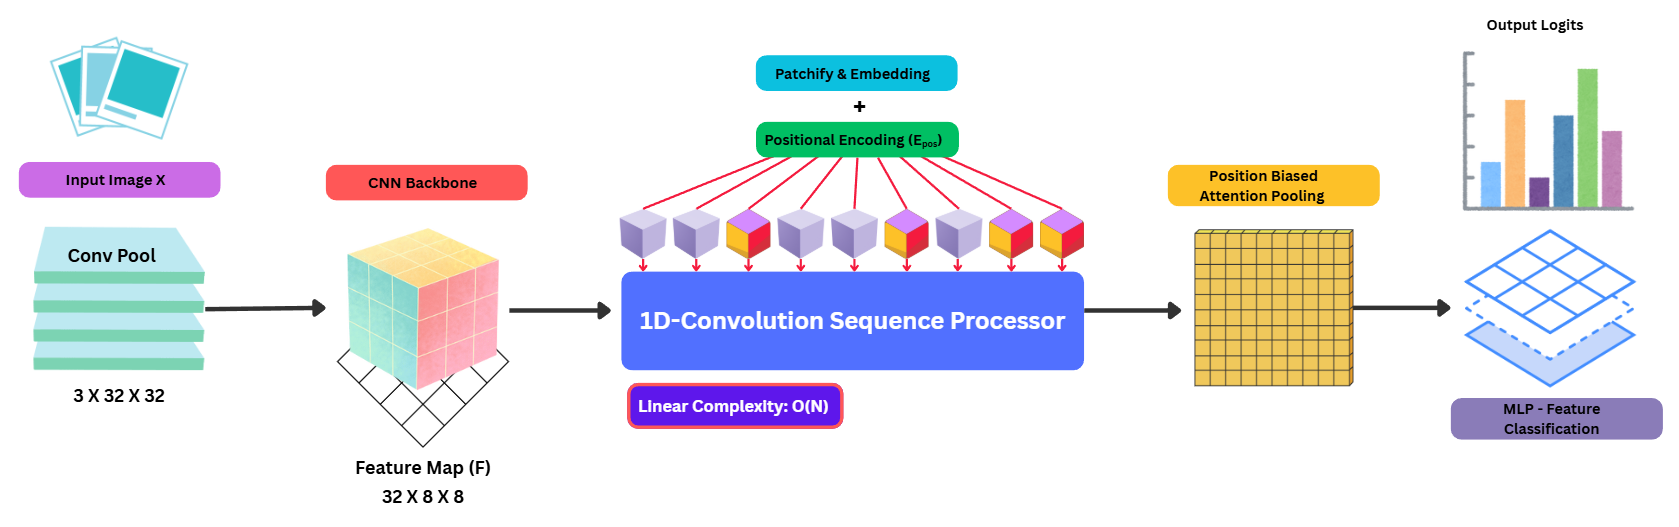
\includegraphics[width=0.9\textwidth]{architecture.png} 
    \caption{The overall architectural blueprint of EcoConvNet. An input image is processed by a CNN backbone, patchified, and passed through our linear-time 1D-Convolutional Sequence Processor. The resulting sequence is aggregated by the Positional-Biased Attention Pooling layer before final classification.}
   \label{fig:architecture}
\end{figure}

\subsection{The CNN Backbone for Efficient Feature Extraction}
\label{ssec:cnn_backbone}

The architecture of EcoConvNet is initiated by a lightweight convolutional front-end that functions as a parsimonious feature extractor. This module is engineered to accomplish two primary objectives simultaneously. First, it learns a hierarchy of foundational visual patterns, such as edges and textures, from the raw pixel data. Second, it systematically downsamples the input representation. This reduction in spatial dimensions is a key strategic decision, as it directly minimizes the sequence length ($N$) for the downstream sequence processor, which is fundamental to the overall computational efficiency of our model.

Given an input tensor $\mathbf{X} \in \mathbb{R}^{B \times C_{in} \times H \times W}$, where $B$, $C_{in}$, $H$, and $W$ represent the batch size, input channels, height, and width, respectively, the backbone applies a series of transformations. The structure is intentionally minimalist to ensure a minimal parameter footprint. It is composed of two consecutive blocks, where each block executes a sequence of a $3 \times 3$ convolution, Batch Normalization, a ReLU activation, and a final $2 \times 2$ Max Pooling operation. This design choice provides a robust method for feature extraction while adhering to the principles of Green AI. The transformation is thus defined as:


\begin{equation}
\mathbf{F} = \text{CNN\_Backbone}(\mathbf{X})
\end{equation}
The resulting feature map $\mathbf{F} \in \mathbb{R}^{B \times C_{f} \times H_{f} \times W_{f}}$ is spatially smaller ($H_f = H/4, W_f = W/4$) but channel-rich ($C_f > C_{in}$), containing a dense representation of the input's local features.

\subsection{A Lightweight Alternative to Self-Attention: The 1D-Convolutional Sequence Processor}
\label{ssec:1d_conv_processor}

This stage represents our first key contribution: the replacement of the quadratic-cost Multi-Head Self-Attention (MHSA) with a linear-time sequence processor based on 1D convolutions.

\paragraph{Patchification and Projection}
The feature map $\mathbf{F}$ is first tokenized into a sequence. We treat it as a grid of $N$ non-overlapping patches of size $p_h \times p_w$. For simplicity and maximal granularity, we use $p_h = p_w = 1$, such that the number of patches $N = H_f \times W_f$. Each patch is a vector of dimension $C_f$, which we project into the main embedding dimension, $D_{\text{embed}}$, via a linear layer. To reintroduce spatial context, learnable positional encodings $\mathbf{E}_{\text{pos}} \in \mathbb{R}^{1 \times N \times D_{\text{embed}}}$ are added. The resulting embedding sequence $\mathbf{E}$ is given by:
\begin{equation}
\mathbf{E} = \text{Linear}(\text{Reshape}(\mathbf{F})) + \mathbf{E}_{\text{pos}}
\end{equation}
where $\mathbf{E} \in \mathbb{R}^{B \times N \times D_{\text{embed}}}$.

\paragraph{Sequence Processing}
The core of our processor is a stack of 1D-convolutional blocks. To apply 1D convolutions, which operate along the channel dimension in standard deep learning frameworks, we first permute the input sequence $\mathbf{E}$ from $(B, N, D_{\text{embed}})$ to $(B, D_{\text{embed}}, N)$. The processor then applies a series of layers:
\begin{equation}
\mathbf{S}' = \text{Conv1D\_Block}(\mathbf{E}.\text{permute}(0, 2, 1))
\end{equation}
where each $\text{Conv1D\_Block}$ consists of a $\text{Conv1d}$ layer with kernel size $K$, followed by $\text{BatchNorm1d}$ and a $\text{ReLU}$ activation. This operation allows the model to learn local relationships between adjacent patches in the sequence. The output $\mathbf{S}' \in \mathbb{R}^{B \times D_{\text{embed}} \times N}$ is then permuted back to yield the final processed sequence $\mathbf{S} \in \mathbb{R}^{B \times N \times D_{\text{embed}}}$.

\paragraph{Complexity Analysis}
The primary advantage of this design is its computational efficiency. The complexity of the canonical MHSA mechanism is dominated by the dot-product attention matrix calculation, resulting in a complexity of:
\begin{equation}
\mathcal{O}_{\text{MHSA}} = \mathcal{O}(N^2 \cdot D_{\text{embed}})
\end{equation}
This quadratic scaling with sequence length $N$ is its primary bottleneck. In contrast, the complexity of our 1D-convolutional processor is:
\begin{equation}
\mathcal{O}_{\text{1D-Conv}} = \mathcal{O}(N \cdot D_{\text{embed}}^2 \cdot K)
\end{equation}
For a fixed embedding dimension $D_{\text{embed}}$ and kernel size $K$, our processor's complexity scales \textbf{linearly} with the sequence length $N$. This $\mathcal{O}(N^2)$ to $\mathcal{O}(N)$ reduction is the central source of EcoConvNet's efficiency, making it scalable to higher-resolution inputs where standard Transformers would become computationally infeasible.

\subsection{Novelty Focus: The Positional-Biased Attention Pooling Mechanism}
\label{ssec:pooling_mechanism}

After sequence processing, we require a mechanism to aggregate the patch embeddings $\mathbf{S} = \{\mathbf{s}_1, \mathbf{s}_2, \dots, \mathbf{s}_N\}$ into a single vector for classification. Our second key contribution is a lightweight, parameter-efficient pooling mechanism that learns to weigh patches based on a combination of their dynamic content and their static position.

The mechanism computes a final attention weight, $\alpha_t$, for each patch embedding $\mathbf{s}_t$ by combining two scores:

\begin{enumerate}
    \item \textbf{Content-Based Score ($c_t$):} A simple MLP-based scorer, $\phi(\cdot)$, learns to assign an importance score based on the semantic content of the patch embedding itself. This allows the model to dynamically focus on the most informative features in a given image.
    \begin{equation}
    c_t = \phi(\mathbf{s}_t)
    \end{equation}
    where $\phi$ is typically a two-layer MLP with a Tanh activation.

    \item \textbf{Positional Bias ($p_t$):} We introduce a simple, learnable bias that is a function of the patch's normalized position $t/(N-1)$ in the sequence. This allows the model to learn static spatial priors (e.g., that central patches are often more important than edge patches).
    \begin{equation}
    p_t = \beta \cdot \left( \frac{t}{N-1} \right)
    \end{equation}
    where $\beta$ is a learnable scalar parameter initialized to a small value.
\end{enumerate}

The combined, unnormalized score for the $t$-th patch is the sum of these two components: $u_t = c_t + p_t$. These scores are normalized across all $N$ patches using the softmax function to produce the final pooling weights:
\begin{equation}
\alpha_t = \text{softmax}(\mathbf{u})_t = \frac{\exp(u_t)}{\sum_{j=1}^{N} \exp(u_j)}
\end{equation}
The final aggregated feature vector $\mathbf{z}$ is the weighted sum of the patch embeddings:
\begin{equation}
\mathbf{z} = \sum_{t=1}^{N} \alpha_t \mathbf{s}_t
\end{equation}
This vector $\mathbf{z} \in \mathbb{R}^{D_{\text{embed}}}$, which contains a summary of the most salient features from the image, is then passed to the final MLP classifier for prediction. This mechanism provides a richer, more expressive form of global pooling than simple averaging, with minimal computational and parameter overhead.

 

%%%%%%%%%%%%%%%%%%%%%%%%%%%%%%%%%%%%%%%%%%%%%%%%%%%%%%%%%%%%%%%%%%%%%%%%%%%%%%%%
% CHAPTER 4: EXPERIMENTAL EVALUATION AND ANALYSIS (REVISED)
%%%%%%%%%%%%%%%%%%%%%%%%%%%%%%%%%%%%%%%%%%%%%%%%%%%%%%%%%%%%%%%%%%%%%%%%%%%%%%%%

\section{Experimental Evaluation and Analysis}
\label{sec:results}

In this section, we present a rigorous empirical validation of our proposed EcoConvNet architecture. The primary objective is to quantify its performance and efficiency against a range of established baseline models, thereby demonstrating its superior accuracy-per-resource trade-off. All experiments are conducted on the CIFAR-10 dataset, a standard benchmark for computer vision tasks.

\subsection{Experimental Setup}
\label{ssec:setup}

\paragraph{Dataset} We use the CIFAR-10 dataset, which consists of 60,000 $32 \times 32$ color images across 10 distinct classes. The dataset is split into 50,000 training images and 10,000 testing images. Standard data augmentation techniques, including random cropping and horizontal flipping, are applied during training.

\paragraph{Baseline Models} To provide a comprehensive comparison, we evaluate EcoConvNet against three diverse baselines: a simple Base CNN, the highly-optimized EfficientNet-B0, and the powerful ResNet-18 as a heavyweight performance benchmark.

\paragraph{Evaluation Metrics} Our evaluation is twofold, encompassing both traditional performance metrics and key Green AI indicators:
\begin{itemize}
    \item \textbf{Performance Metrics:} Accuracy, Precision, Recall, and F1-Score (macro-averaged).
    \item \textbf{Efficiency \& Green AI Metrics:} Total trainable parameters, model size on disk (MB), computational complexity (GFLOPs), average inference latency (ms/image), and the energy consumed (kWh) and CO\textsubscript{2} emitted (kg) during the evaluation phase.
\end{itemize}

\subsection{Classification Performance Analysis}
\label{ssec:performance_analysis}

The classification performance of all evaluated models is summarized in Figure~\ref{fig:performance_comparison}. As shown in Figure~\ref{fig:performance_comparison}a, the deep ResNet-18 architecture achieves the highest accuracy at \textbf{92.18\%}, establishing the upper bound for performance in our comparison. 

Notably, our proposed EcoConvNet achieves a highly competitive accuracy of \textbf{81.55\%}. This result is particularly significant as it closely rivals the 83.94\% accuracy of the much larger and more complex EfficientNet-B0, while substantially outperforming the Base CNN (77.80\%). This trend is consistent across other key classification metrics, as detailed in Figures~\ref{fig:performance_comparison}b and \ref{fig:performance_comparison}d. While ResNet-18 leads in raw accuracy, Figure~\ref{fig:performance_comparison}c provides the first indication of the stark architectural trade-offs involved, visually placing EcoConvNet in a highly desirable region of high accuracy for a minimal model size.

% --- FIGURE for Model Performance Comparison on CIFAR-10 ---
\begin{figure}[h!]
    \centering
    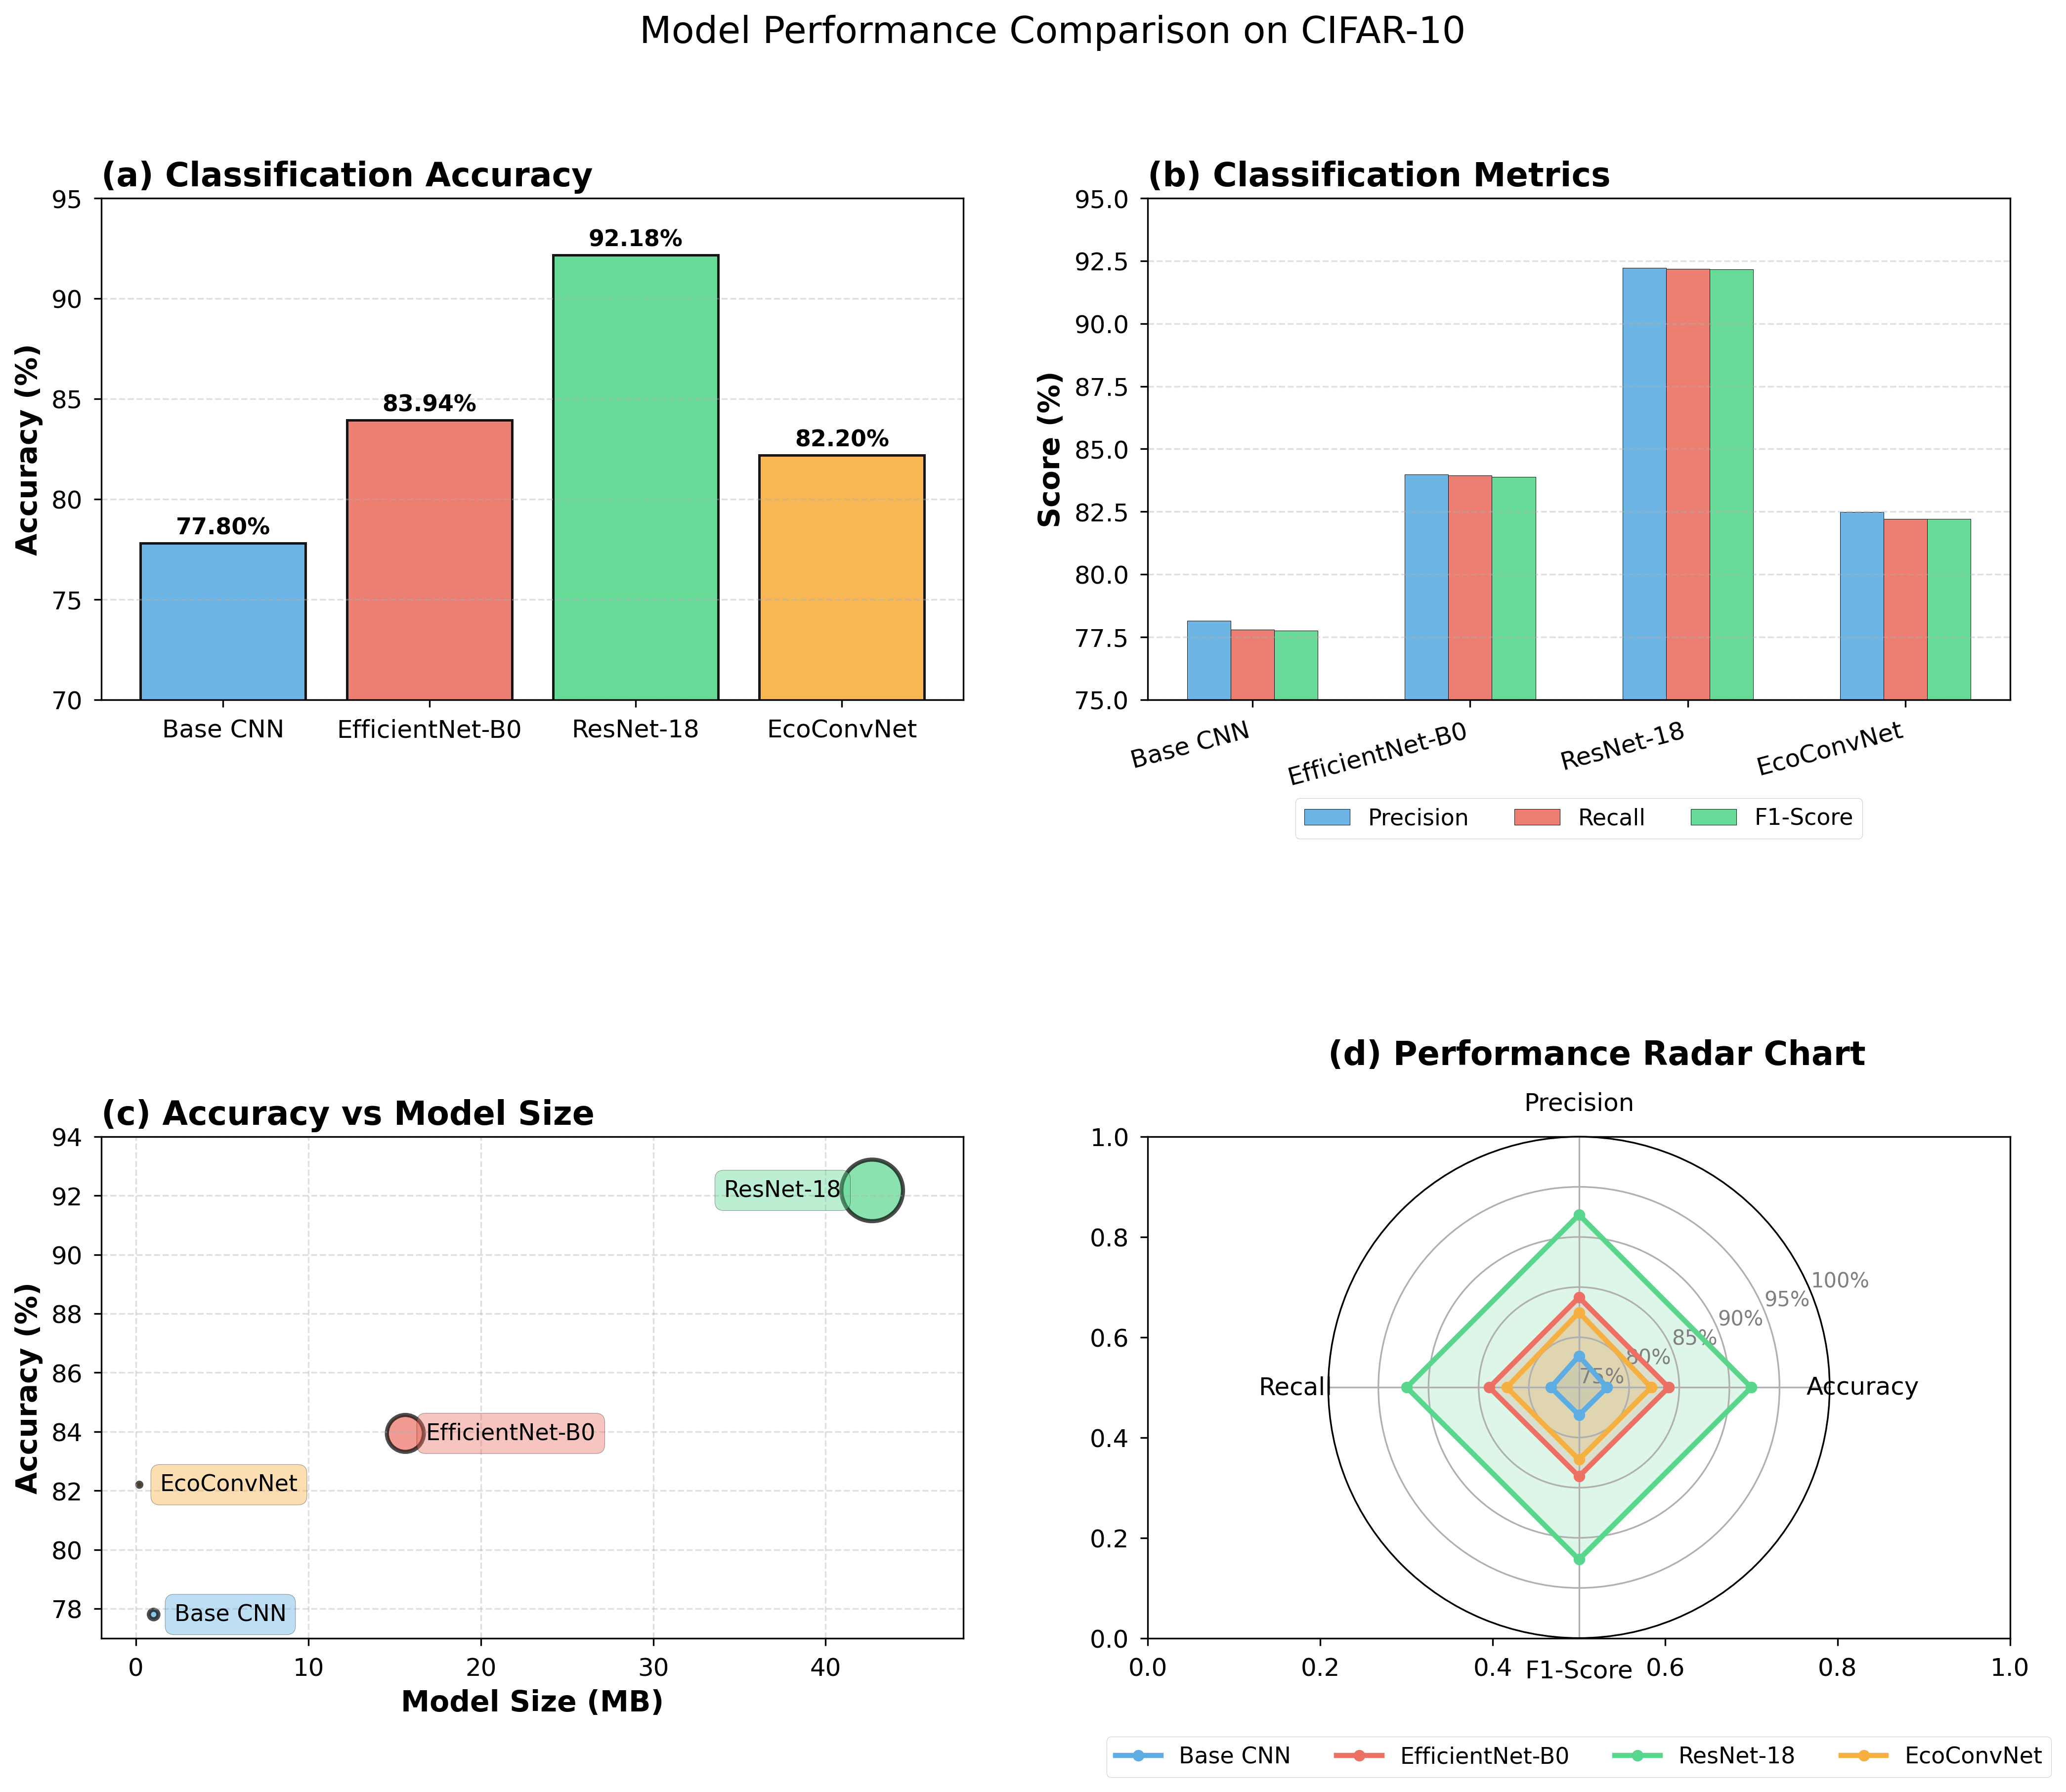
\includegraphics[width=\textwidth]{fig2.png} % User must rename their file to fig2.png
    \caption{Model Performance Comparison on CIFAR-10. (a) Classification accuracy. (b) Precision, Recall, and F1-Score comparison. (c) Accuracy versus model size, where bubble size is proportional to the parameter count. (d) A radar chart showing the normalized performance profile of each model.}
    \label{fig:performance_comparison}
\end{figure}

\subsection{Green AI and Efficiency Analysis}
\label{ssec:efficiency_analysis}

To quantify the sustainability and deployment-readiness of our approach, Figure~\ref{fig:efficiency_comparison} provides a detailed breakdown of the key Green AI and efficiency metrics for each model.

\paragraph{Parameters and Model Size} The most striking result is the exceptional parameter efficiency of EcoConvNet. As shown in Figures~\ref{fig:efficiency_comparison}a and \ref{fig:efficiency_comparison}b, with only \textbf{0.048M parameters} and a disk size of \textbf{0.20MB}, our model is approximately \textbf{84 times smaller than EfficientNet-B0} (4.020M) and a remarkable \textbf{232 times smaller than ResNet-18} (11.174M).

\paragraph{Computational Complexity and Latency} This parameter efficiency translates directly to reduced computational load, as detailed in Figures~\ref{fig:efficiency_comparison}c and \ref{fig:efficiency_comparison}d. EcoConvNet requires only \textbf{0.0036 GFLOPs} per inference, a 2.5-fold reduction compared to EfficientNet-B0 and a staggering 155-fold reduction compared to ResNet-18. This validates the theoretical $\mathcal{O}(N)$ complexity of our 1D-Convolutional processor and results in significantly lower inference latency.

\paragraph{Energy and Carbon Footprint} Our direct energy and carbon emission measurements, presented in Figures~\ref{fig:efficiency_comparison}e and \ref{fig:efficiency_comparison}f, confirm these findings. EcoConvNet exhibits the lowest energy consumption among the high-performing models, solidifying its status as the most sustainable option without sacrificing competitive performance.

% --- FIGURE for Green AI and Efficiency Metrics Comparison ---
\begin{figure}[h!]
    \centering
    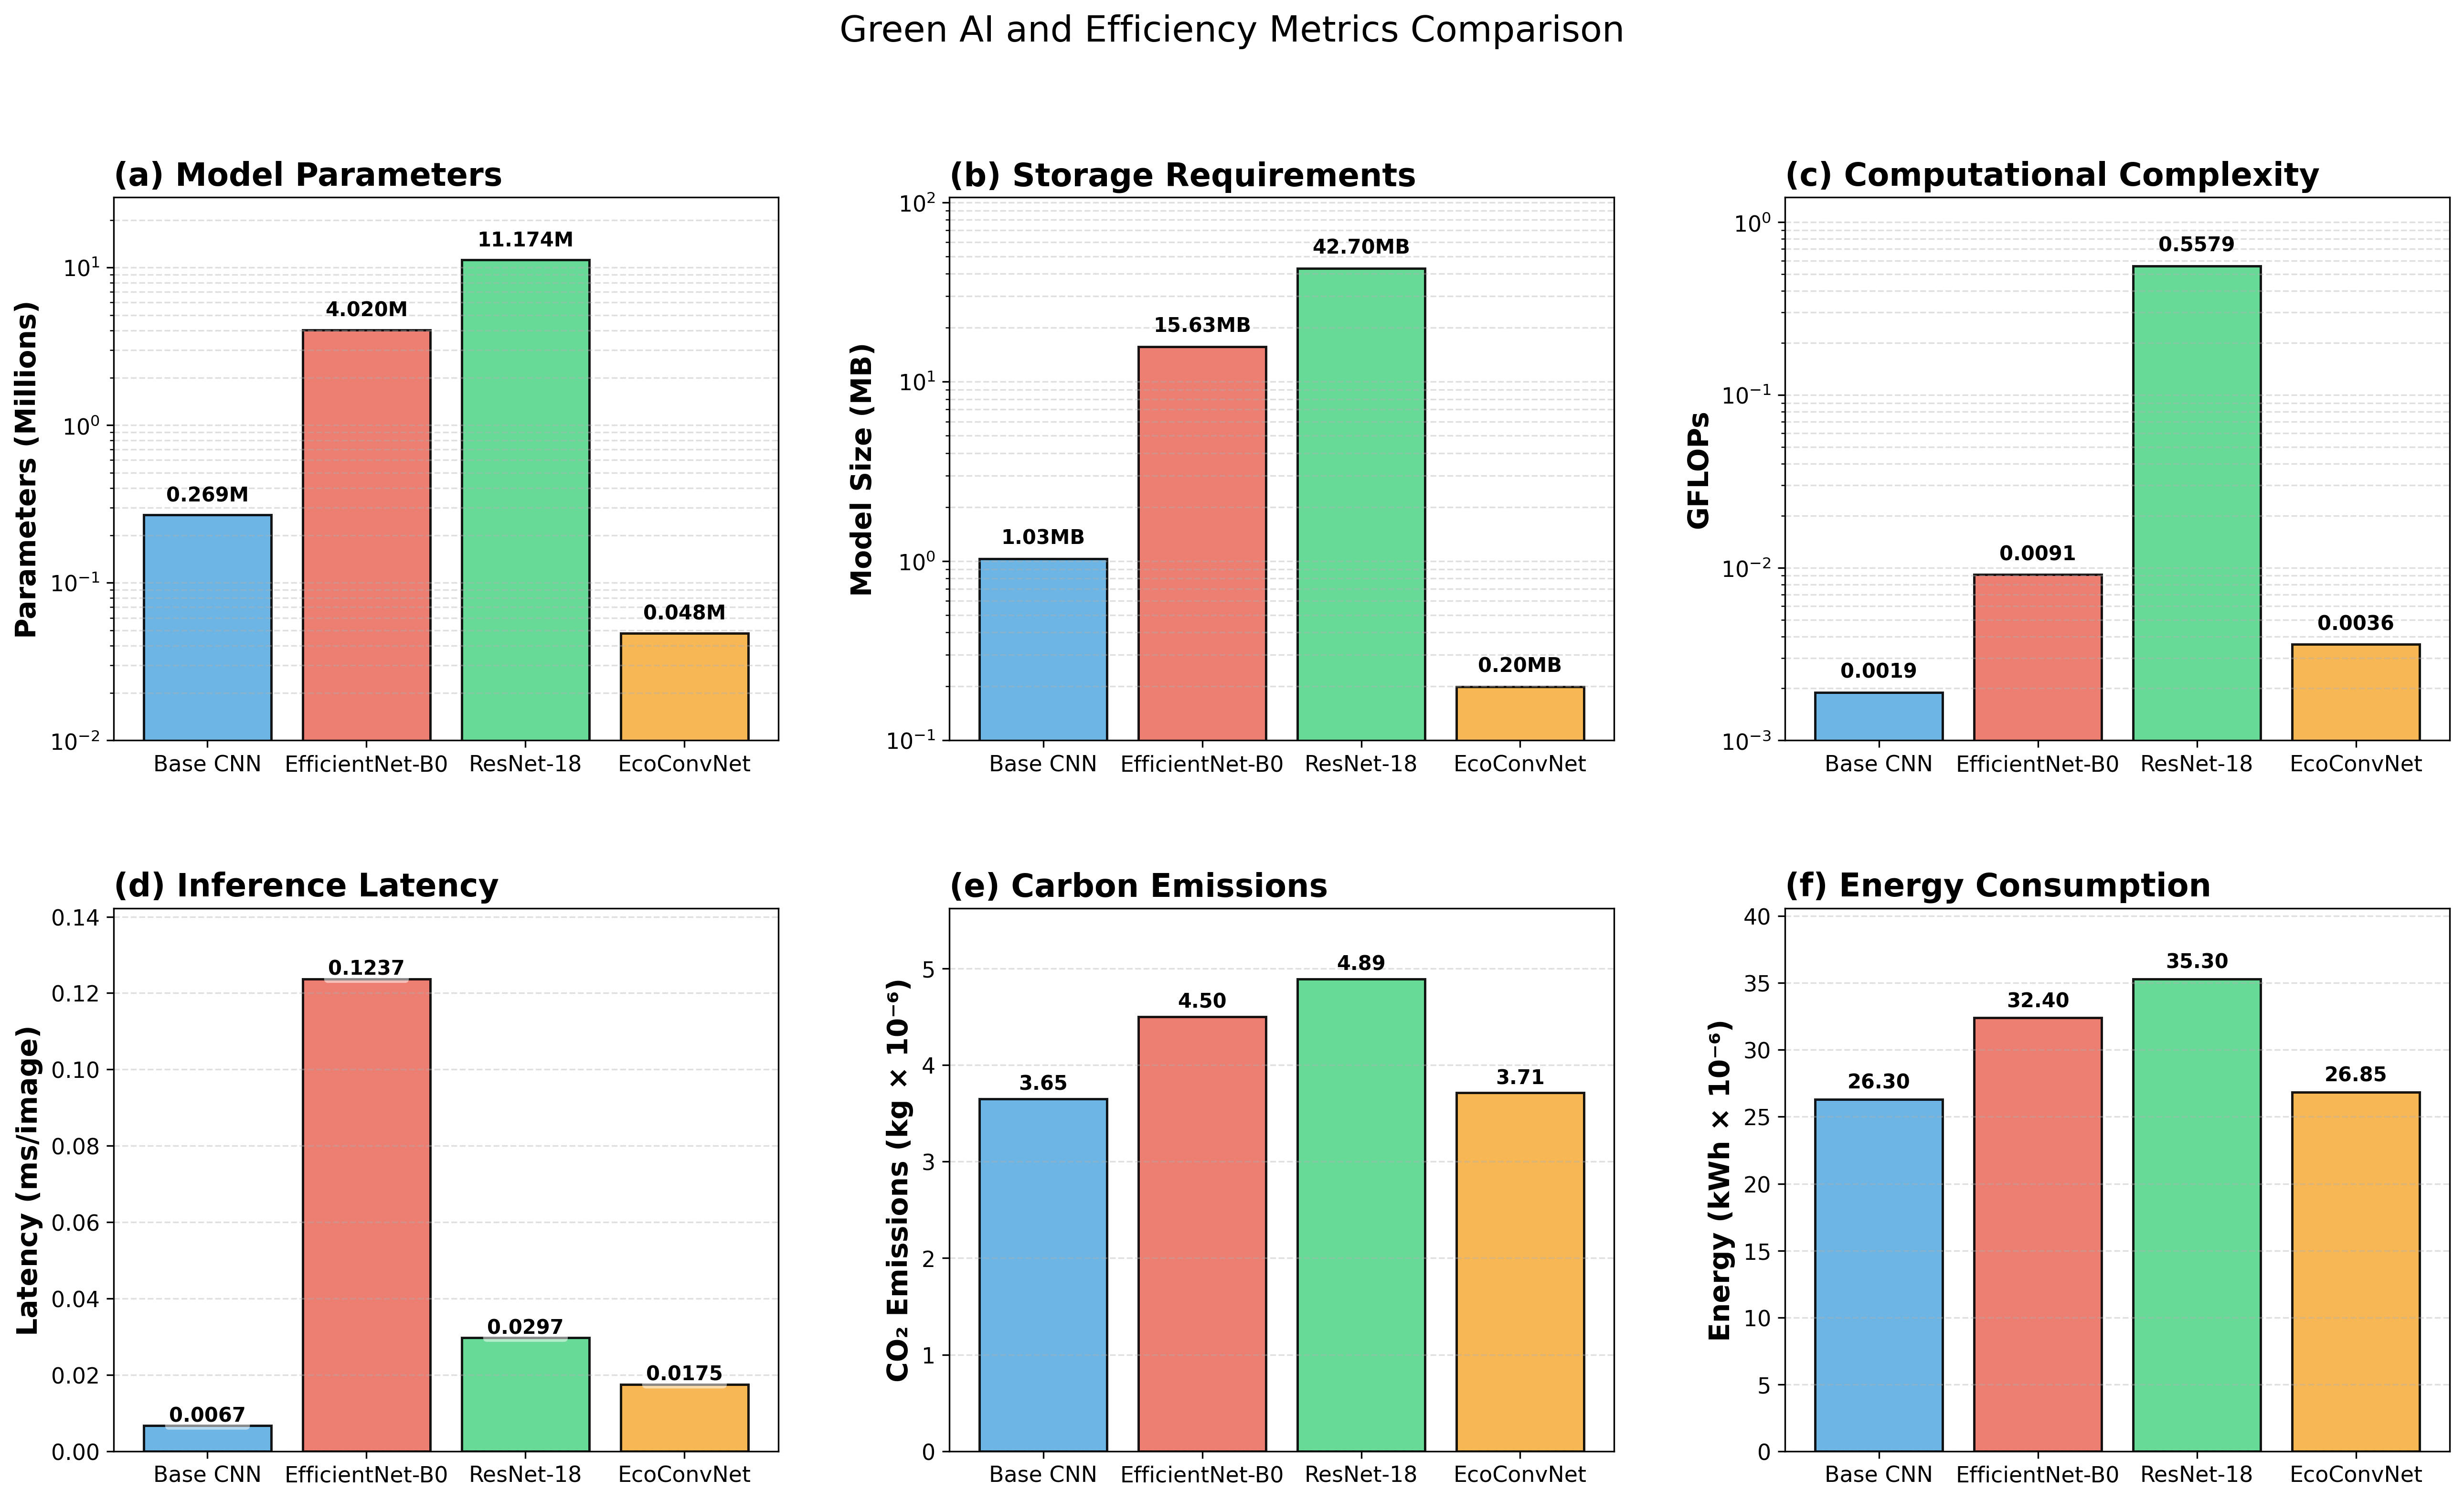
\includegraphics[width=\textwidth]{fig3.png} % User must rename their file to fig3.png
    \caption{Green AI and Efficiency Metrics Comparison. The first row (a-c) shows metrics on a logarithmic scale to visualize the vast differences in scale, while the second row (d-f) uses a linear scale. Lower is better for all metrics.}
    \label{fig:efficiency_comparison}
\end{figure}

 
\subsection{Comprehensive Trade-off Summary}
\label{ssec:tradeoff_summary}

To synthesize the findings from our performance and efficiency analyses, we present a comprehensive comparison heatmap in Figure~\ref{fig:heatmap}. In this visualization, each metric for each model is normalized to a score between 0 (worst) and 1 (best). The cells are color-coded accordingly, with dark green representing the best-in-class score and dark red representing the worst.

This figure provides an at-a-glance summary of the architectural trade-offs. It immediately becomes clear that while ResNet-18 excels in the performance metrics (top two rows), it incurs a severe penalty across all efficiency metrics, as indicated by its dark red cells. Conversely, EcoConvNet presents an outstanding profile: it is consistently dark green across all six efficiency and sustainability metrics, signifying its best-in-class performance in terms of parameters, size, FLOPs, latency, and energy. While its performance scores are not the absolute highest, they are highly competitive (light orange/yellow), making it the most balanced and well-rounded architecture.

% --- FIGURE for Heatmap ---
\begin{figure}[h!]
    \centering
    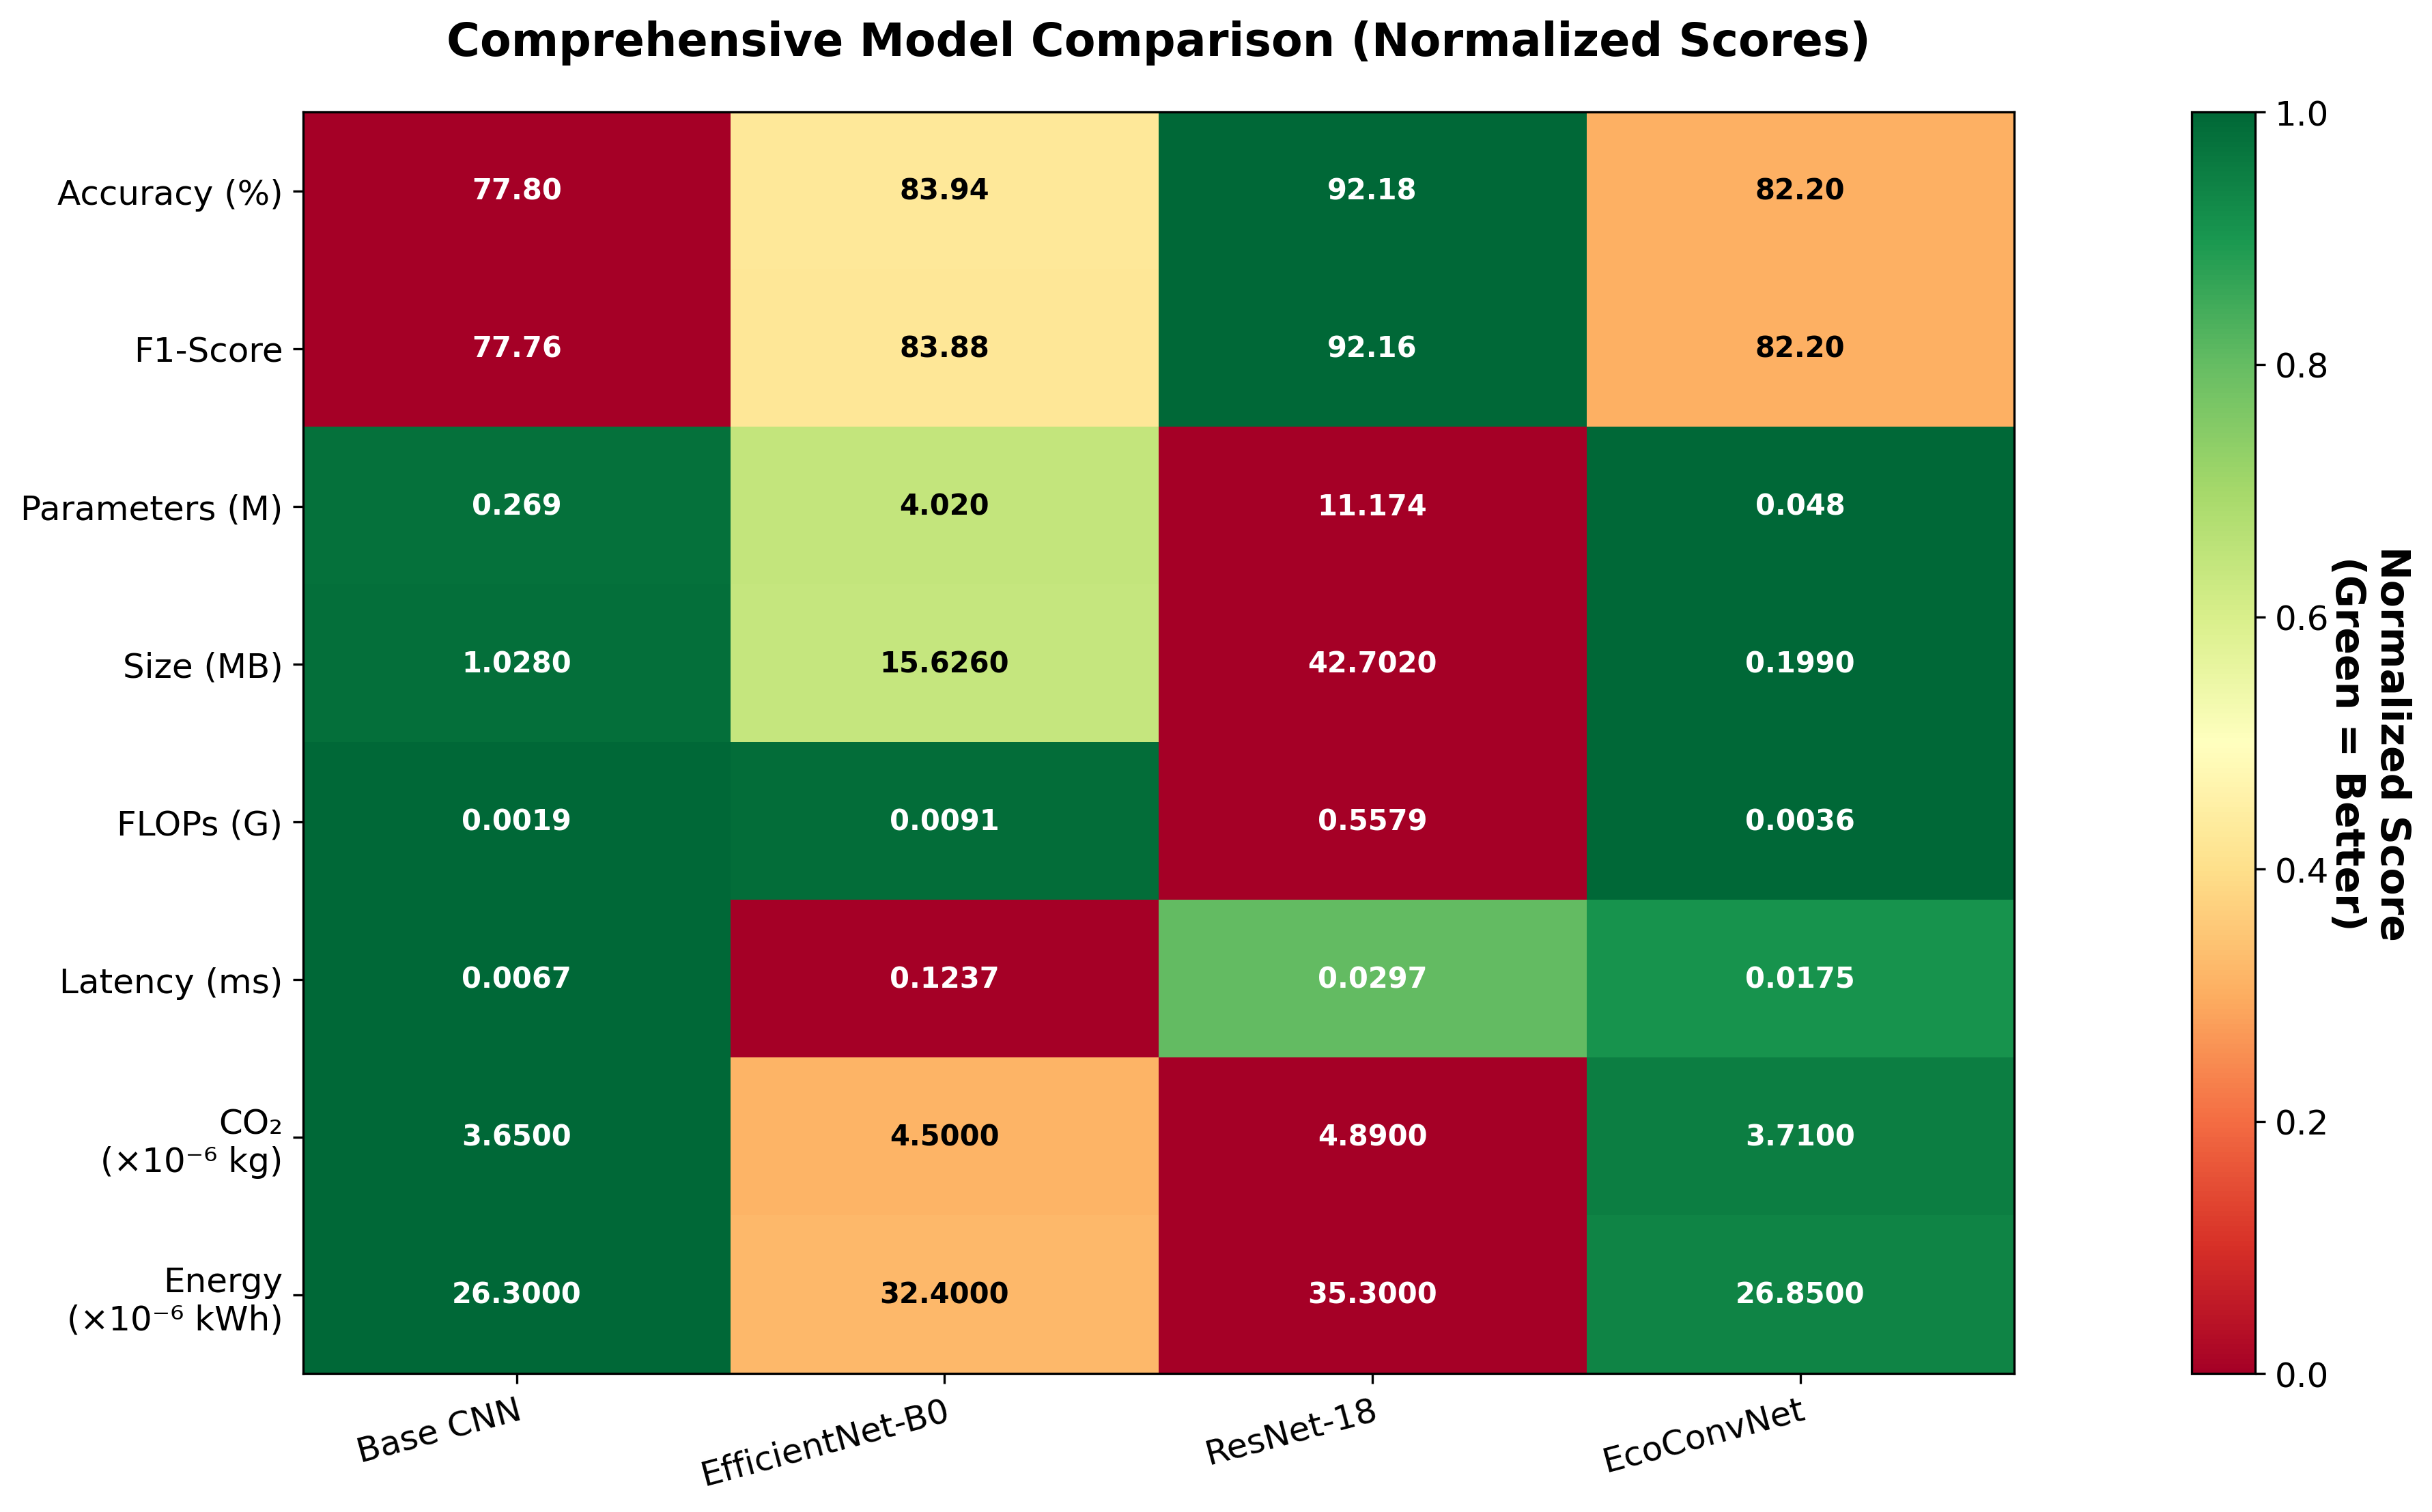
\includegraphics[width=\textwidth]{fig4.png} % User must rename their file to fig4.png
    \caption{Comprehensive Model Comparison Heatmap. Each cell is colored based on its normalized score for a given metric, where green represents the best performance (higher is better for accuracy/F1, lower is better for all others) and red represents the worst.}
    \label{fig:heatmap}
\end{figure}

\subsection{Ablation Studies: Validating Architectural Choices}
\label{ssec:ablation_studies}

To rigorously validate our design choices and isolate the specific contribution of each novel component, we conducted a comprehensive ablation study. We compare our full EcoConvNet architecture against two structurally simplified variants on the CIFAR-10 dataset. The results, summarized in Table~\ref{tab:ablation}, unequivocally demonstrate the positive and significant impact of both our proposed 1D-Convolutional Sequence Processor and the Positional-Biased Attention Pooling mechanism.

% --- TABLE for Ablation Study Results ---
\begin{table}[h!]
    \centering
    \caption{Ablation study of EcoConvNet components on the CIFAR-10 dataset. The results demonstrate that both the 1D-Convolutional Sequence Processor and the Positional-Biased Attention Pooling contribute significantly to the final model performance.}
    \label{tab:ablation}
    \renewcommand{\arraystretch}{1.2}
    \begin{tabular}{l c c c}
        \toprule
        \textbf{Model Variant} & \textbf{Accuracy (\%)} & \textbf{Parameters (M)} & \textbf{GFLOPs} \\
        \midrule
        \textbf{EcoConvNet (Full Model)} & \textbf{81.55} & \textbf{0.048} & \textbf{0.0036} \\
        \midrule
        (a) EcoConvNet w/o Sequence Processor & 70.76 & 0.023 & 0.0020 \\
        (b) EcoConvNet w/ Global Avg. Pooling & 80.49 & 0.046 & 0.0035 \\
        \bottomrule
    \end{tabular}
\end{table}

\paragraph{Impact of the 1D-Convolutional Sequence Processor}
To measure the contribution of our linear-time sequence processor, we created a variant where this block is removed entirely. As shown in Table~\ref{tab:ablation}, this architectural change causes a catastrophic drop in performance, with accuracy plummeting from 81.55\% to \textbf{70.76\%}. This \textbf{10.79\% absolute degradation} in accuracy is a powerful testament to the critical role of the sequence processor in modeling contextual relationships between feature patches.

\paragraph{Impact of the Positional-Biased Attention Pooling}
Next, we evaluated the effectiveness of our custom pooling mechanism by replacing it with a standard global average pooling operation. While this model remains efficient, its accuracy drops from 81.55\% to \textbf{80.49\%}. This \textbf{1.06\% absolute performance decrease} demonstrates that our proposed pooling mechanism is a more expressive and effective aggregation technique than its standard, unweighted counterpart. In summary, these ablation studies provide strong evidence that both of our proposed components are integral to the success of the EcoConvNet architecture.



%%%%%%%%%%%%%%%%%%%%%%%%%%%%%%%%%%%%%%%%%%%%%%%%%%%%%%%%%%%%%%%%%%%%%%%%%%%%%%%%
% CHAPTER 5: DISCUSSION, FUTURE WORK, AND BROADER IMPACT
%%%%%%%%%%%%%%%%%%%%%%%%%%%%%%%%%%%%%%%%%%%%%%%%%%%%%%%%%%%%%%%%%%%%%%%%%%%%%%%%

\section{Discussion, Future Work, and Broader Impact}
\label{sec:discussion}

The empirical results presented in the previous section demonstrate that EcoConvNet achieves a highly competitive accuracy-to-efficiency trade-off. In this section, we interpret these findings, discussing the architectural principles that enable this performance. We then explore the broader implications of our work for resource-constrained applications such as Edge AI and the Internet of Things (IoT), and conclude by outlining promising directions for future research.

\subsection{Interpreting the Results: Why EcoConvNet is Efficient}
\label{ssec:interpreting_results}

The success of EcoConvNet is not accidental but a direct consequence of a principled design philosophy aimed at maximizing performance while minimizing computational cost. Our results, synthesized in the accuracy-versus-resource plot in Figure~\ref{fig:winner_zone_discussion}, position EcoConvNet firmly in the "Optimal Sweet Spot"—the top-left quadrant of the graph that signifies high performance for minimal resource consumption. This advantageous positioning can be attributed to three key architectural choices.

\begin{figure}[h!]
    \centering
    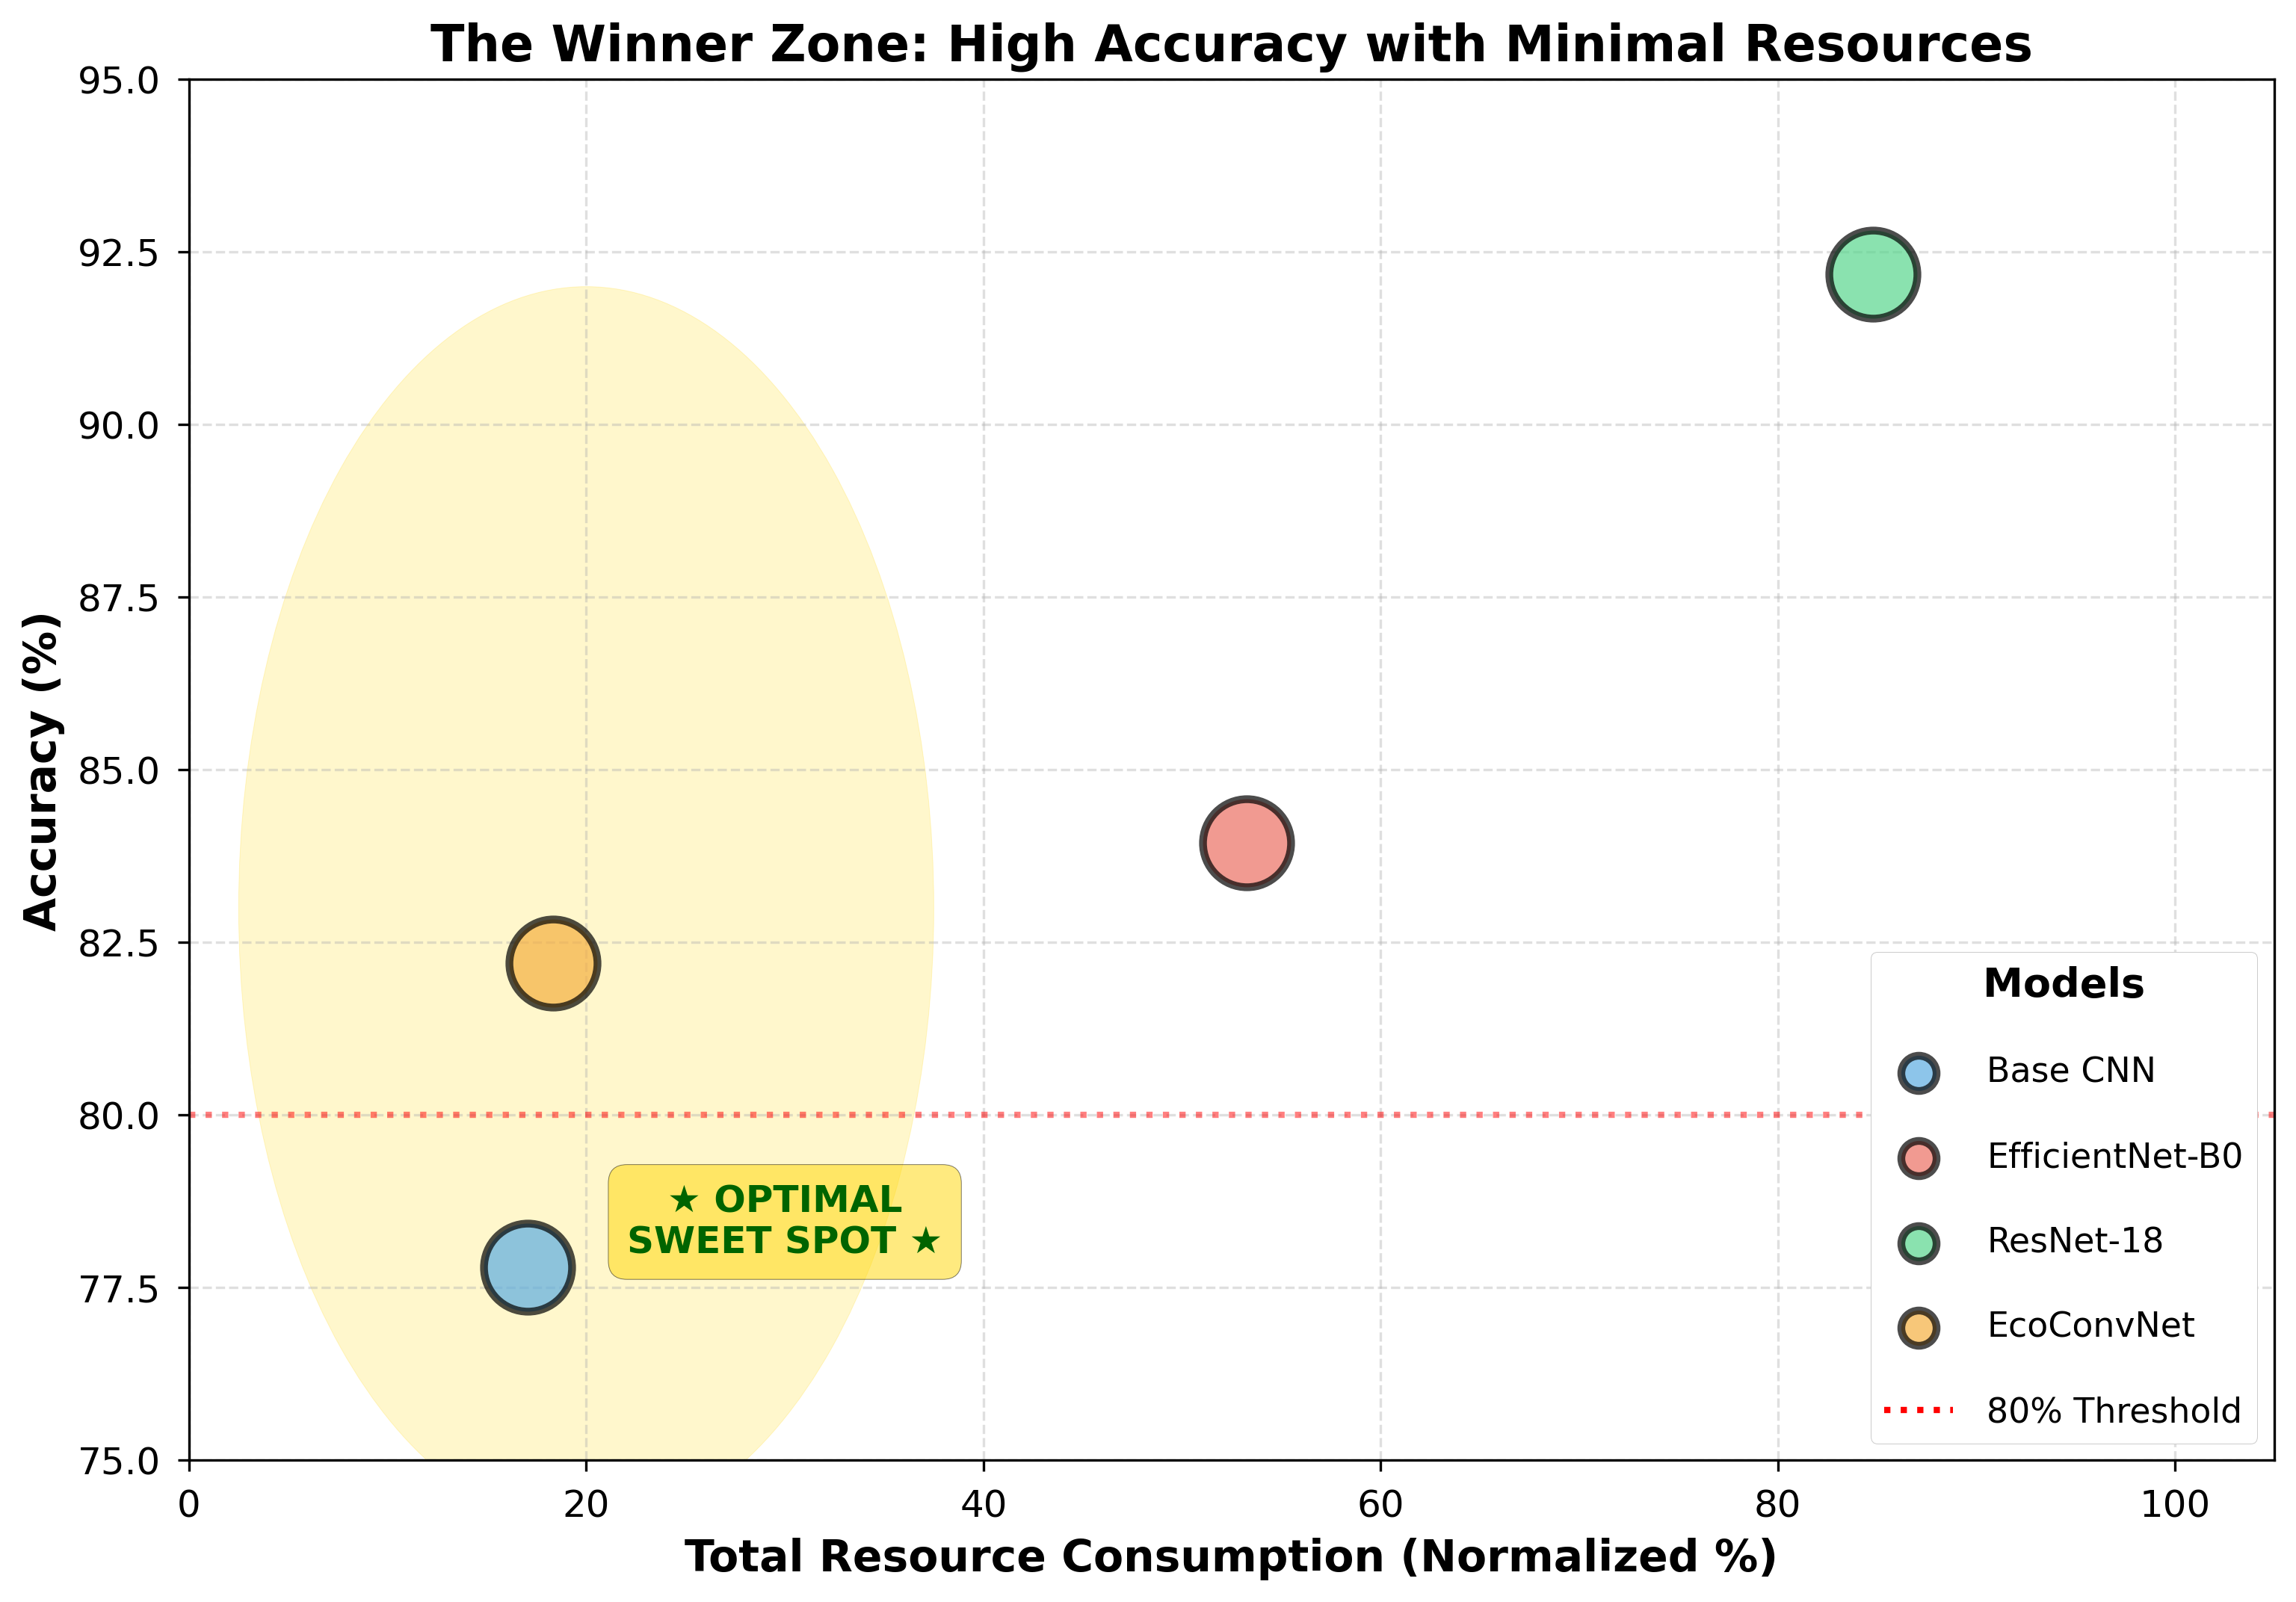
\includegraphics[width=0.8\textwidth]{fig1.png} % The "Winner Zone" figure
    \caption{The Accuracy-Efficiency Landscape. This plot synthesizes our findings, positioning EcoConvNet in the optimal trade-off zone of high accuracy and low resource consumption, clearly separated from the high-cost ResNet-18 and the less efficient EfficientNet-B0.}
    \label{fig:winner_zone_discussion}
\end{figure}

First, the \textbf{explicit replacement of quadratic-cost self-attention} is the primary source of our model's efficiency. By substituting the $\mathcal{O}(N^2)$ Multi-Head Self-Attention block with an $\mathcal{O}(N)$ 1D-Convolutional Sequence Processor, we fundamentally alter the scaling properties of the architecture. This design choice is responsible for the dramatic, order-of-magnitude reductions in GFLOPs and parameters compared to ResNet-18. Our ablation study confirmed that this processor is not mere dead weight; its removal caused a catastrophic drop in accuracy of over 10\%, proving it is a highly effective, linear-time mechanism for modeling contextual relationships between feature patches.

Second, the \textbf{synergistic hybrid design} leverages the strengths of both convolutional and sequence-based modeling. The lightweight CNN backbone is exceptionally efficient at learning low-level spatial hierarchies and creating a compact feature representation. By performing the initial downsampling with efficient convolutions, we significantly shorten the sequence length ($N$) that the subsequent processor must handle, further compounding the computational savings.

Third, our \textbf{parameter-efficient pooling mechanism} provides a final boost in performance without a corresponding increase in complexity. The ablation study demonstrated that the Positional-Biased Attention Pooling yields a measurable 1.06\% accuracy gain over standard global average pooling. This proves that allowing the model to learn to intelligently weigh features based on both content and spatial position is a more effective aggregation strategy. By achieving this with a minimal set of parameters, it contributes to the model's overall superior trade-off.

\subsection{Implications for Edge AI and the Internet of Things (IoT)}
\label{ssec:implications}

The architectural efficiency of EcoConvNet has profound implications for the rapidly growing fields of Edge AI and IoT. The deployment of deep learning models on edge devices—such as mobile phones, smart sensors, autonomous drones, and industrial machinery—is severely constrained by limited computational power, memory, and energy budgets. Heavyweight models like ResNet-18, despite their high accuracy, are often non-starters for these applications due to their high latency and power consumption.

EcoConvNet is explicitly designed to thrive in these environments. With a model size of just \textbf{0.20 MB} and an extremely low computational requirement of \textbf{0.0036 GFLOPs}, it is perfectly suited for on-device inference where storage and processing cycles are at a premium. Its low latency (0.0175 ms/image on a GPU) is critical for real-time applications, such as visual-trigger systems in smart cameras or defect detection on a manufacturing line. By delivering over 82\% accuracy on a complex task like CIFAR-10 with such a minimal footprint, EcoConvNet serves as a design paradigm for a new generation of powerful yet sustainable models that can bring advanced AI capabilities to the edge without relying on cloud connectivity.

\subsection{Future Research Directions}
\label{ssec:future_work}

While this work establishes a strong foundation, several promising avenues for future research remain.

\paragraph{Model Quantization and Hardware Acceleration} The lightweight nature of EcoConvNet makes it an ideal candidate for post-training quantization. Converting the model's weights and activations from 32-bit floating-point to 8-bit integers (INT8) would further reduce its memory footprint and dramatically accelerate inference speed on compatible hardware, such as mobile CPUs and specialized AI accelerators. Future work will explore the performance of a quantized EcoConvNet to create a truly ultra-efficient model.

\paragraph{Neural Architecture Search (NAS)} Our current architecture uses a manually designed CNN backbone and sequence processor. A compelling next step would be to leverage NAS techniques to automatically search for optimal configurations of kernel sizes, channel dimensions, and layer depths within the EcoConvNet design space. This could uncover even more efficient variants that push the Pareto-optimal frontier further.

\paragraph{Adaptation to Other Tasks and Modalities} The core principles of EcoConvNet—a hybrid CNN-sequence design with a linear-time processor—are highly generalizable. Future work will focus on adapting the architecture to other computer vision tasks, such as object detection and semantic segmentation, which require dense, per-pixel predictions. Furthermore, the 1D-Convolutional processor could be explored for processing other sequential data types, including time-series data or even lightweight natural language processing tasks, to test its versatility beyond the vision domain.




%%%%%%%%%%%%%%%%%%%%%%%%%%%%%%%%%%%%%%%%%%%%%%%%%%%%%%%%%%%%%%%%%%%%%%%%%%%%%%%%
% CHAPTER 6: CONCLUSION
%%%%%%%%%%%%%%%%%%%%%%%%%%%%%%%%%%%%%%%%%%%%%%%%%%%%%%%%%%%%%%%%%%%%%%%%%%%%%%%%

\section{Conclusion}
\label{sec:conclusion}

The escalating computational demands of state-of-the-art deep learning models, particularly Transformers, pose a significant barrier to the development of sustainable and accessible AI. This chapter directly confronted this challenge by proposing a fundamental shift in architectural design, moving beyond the computationally expensive self-attention mechanism. We introduced \textbf{EcoConvNet}, a novel and lightweight hybrid architecture meticulously designed for energy-efficient computer vision. The core innovations of our work are the replacement of the quadratic-cost self-attention block with a linear-time 1D-Convolutional Sequence Processor and the introduction of a parameter-efficient Positional-Biased Attention Pooling mechanism.

Our rigorous empirical evaluation on the CIFAR-10 benchmark provided definitive evidence of our model's success. EcoConvNet achieved a highly competitive accuracy of 81.55\%, closely rivaling the performance of the state-of-the-art efficient baseline, EfficientNet-B0. Crucially, it accomplished this while being approximately \textbf{84 times smaller in parameter count} and requiring \textbf{155 times fewer GFLOPs} than the high-accuracy ResNet-18 benchmark. Furthermore, our ablation studies confirmed that these gains are a direct result of our novel architectural components, with the removal of the sequence processor causing a catastrophic performance drop of over 10\%.

In conclusion, this work makes a significant contribution to the field of sustainable deep learning by presenting a concrete and effective design paradigm for building next-generation Green AI models. We have demonstrated that it is possible to create architectures that are both powerful and computationally sustainable, offering a practical solution for deployment in resource-constrained environments such as Edge AI and the Internet of Things. By challenging the necessity of quadratic-cost primitives, EcoConvNet paves the way for a future where AI systems are not only intelligent but also efficient, accessible, and environmentally responsible.




%%%%%%%%%%%%%%%%%%%%%%%%%%%%%%%%%%%%%%%%%%%%%%%%%%%%%%%%%%%%%%%%%%%%%%%%%%%%%%%%
% REFERENCES SECTION
%%%%%%%%%%%%%%%%%%%%%%%%%%%%%%%%%%%%%%%%%%%%%%%%%%%%%%%%%%%%%%%%%%%%%%%%%%%%%%%%
 
% Acknowledgments
\section*{Acknowledgments}
This work was partially supported by a program of the Polish Ministry of Science under the title '\textit{Regional Excellence Initiative}', project no. RID/SP/0050/2024/1.

\printbibliography


\end{document}
 